\documentclass[11pt]{article}
\usepackage[utf8]{inputenc}
\usepackage[T1]{fontenc}
\usepackage{geometry}
\usepackage{amsmath}
\usepackage{amsfonts}
\usepackage{amssymb}
\usepackage{graphicx}
% \usepackage{natbib}
\usepackage{url}
\usepackage{hyperref}
\usepackage{titlesec}
\usepackage{enumitem}
\usepackage{wrapfig}
\usepackage[backend=biber]{biblatex}
\addbibresource{ref.bib}

\usepackage{booktabs}
\usepackage{array}
\usepackage{caption}
\usepackage{subcaption}
\usepackage{lmodern}
\usepackage{microtype}
\usepackage{threeparttable}   % for threeparttable and tablenotes
\captionsetup{font=scriptsize, labelfont=bf, position=top, skip=3pt}
\setlength{\tabcolsep}{4pt}
\renewcommand{\arraystretch}{1.05}

% Page layout
\geometry{
    left=0.8in,
    right=0.6in,
    top=0.6in,
    bottom=0.8in
}
\newcommand{\ts}{\mathrm{TS}}
\newcommand{\jsd}{\mathrm{JSD}}
\newcommand{\tsw}{\mathrm{TS_{wild}}}
\newcommand{\inm}{\mathrm{Infl}}
\newcommand{\adj}{\mathrm{Adj}}
\newcommand{\K}[1]{{\color{red}[[\textbf{K: }#1]]}}
\newcommand{\E}[1]{{\color{blue}#1}}
\newcommand{\facin}{f(\mathrm{act/inh})}
\newcommand{\ewnum}{\mathrm{EW_{num}}}
\newcommand{\tsten}{\mathrm{Toggle Switch (10N,100E)}}
\newcommand{\tstwo}{\mathrm{Toggle Switch (10N,80E)}}
\newcommand{\tsfour}{\mathrm{Toggle Switch (10N,60E)}}
\newcommand{\tssix}{\mathrm{Toggle Switch (10N,40E)}}
\newcommand{\tseight}{\mathrm{Toggle Switch (10N,20E)}}
\newcommand{\emttwosix}{\mathrm{EMT (23N,89E)}}
\newcommand{\emtrac}{\mathrm{EMT (17N,62E)}}
\newcommand{\gonad}{\mathrm{Gonadal (18N,74E)}}
\newcommand{\siltwo}{\mathrm{Silviera (18N,37E)}}
\newcommand{\sil}{\mathrm{Silviera (16N,30E)}}
\newcommand{\sclc}{\mathrm{SCLC (33N,357E)}}
\newcommand{\tennode}{\mathrm{NRF2 + OVOL (8N,19E)}}
\newcommand{\twenode}{\mathrm{NRF2 + GRHL2 + OVOL (11N,28E)}}
\newcommand{\beginsupplement}{%
        \setcounter{table}{0}
        \renewcommand{\thetable}{S\arabic{table}}%
        \setcounter{figure}{0}
        \renewcommand{\thefigure}{S\arabic{figure}}%
        \setcounter{section}{0}
        \renewcommand{\thesection}{S\arabic{section}}%
     }

%%%%%%%%%%%%%%%%%%%%%%%%%%%%%%%%%%%%%%%%%%%%%%%%%%
\title{Regulatory stochasticity drives opposing phenotypic outcomes in cell-fate decision networks\\
\vspace{5pt}
Contrasting phenotypic outcomes arising from regulatory stochasticity in cell-fate decision networks\\
}

\author{Abhay Gupta, Lakshmi Malvadi, Prakash Kulkarni, Ravi Salgia, Herbert Levine, \\ Mohit Kumar Jolly, Kishore Hari}

\begin{document}

\maketitle

\begin{abstract}
Gene regulatory networks (GRNs) underlying cell-fate decisions are conventionally modelled as deterministic systems with fixed interaction parameters, yet the effective strength of any regulatory interaction fluctuates continuously in vivo. Intrinsically disordered regions in transcription factors, non-specific genomic binding sites, and stochastic enhancer dynamics collectively introduce temporal variability in the fold-change parameters that govern regulatory efficacy --- a form of structural stochasticity that is distinct from, and largely independent of, classical copy-number noise. How such parameter-level noise shapes the emergent phenotypic landscape of cell-fate circuits remains poorly understood. Here, we systematically evaluate the effects of three modes of structural noise --- additive (state-independent), multiplicative (state-dependent), and stationary (mean-reverting) --- on GRN motifs underlying binary and tertiary cell-fate decisions. Using RACIPE-generated parameter ensembles, we simulate toggle switches, toggle switches with self-activation, and toggle triads under each noise mode across a wide range of noise magnitudes, and extend the analysis to larger binary cell-fate networks governing epithelial--mesenchymal transition and gonadal cell-fate determination using a Boolean framework. Additive noise consistently drives networks away from terminal attractors toward hybrid co-expression states, with the effect scaling with noise intensity and being strongest in bistable parameter regimes and sparser network architectures. Multiplicative noise, by contrast, reinforces inhibitory interactions over time and stabilises terminal phenotypes across all topologies studied. Stationary noise produces minimal disruption to the phenotypic landscape, consistent with a normal physiological baseline. These results establish that the type of structural noise, not only its magnitude, is a key determinant of phenotypic plasticity in cell-fate circuits, and suggest that additive-like noise --- plausibly arising from IDR conformational dynamics or open chromatin in stem cells --- may be a non-genetic driver of hybrid state enrichment and intra-tumour heterogeneity.
\end{abstract}

\section{Introduction}\label{sec:Intro}

Gene regulatory networks (GRNs) are conventionally modelled as deterministic systems with fixed interaction parameters, yet the effective strength of any regulatory interaction is subject to continuous fluctuation in vivo. Transcription factors are enriched in intrinsically disordered regions (IDRs) that mediate conformationally heterogeneous, PTM-sensitive contacts with DNA and co-factors, causing regulatory affinities to vary dynamically rather than assume a fixed value \cite{Ferrie2022Structure-functionRegulation, Holehouse2023TheRegions}. Non-specific TF binding to genomic decoy sites further modulates the effective regulatory signal in an affinity- and abundance-dependent manner \cite{Dey2020EnhancementSites, Burger2012InfluenceExpression}. Enhancer dynamics and transcriptional bursting add a third layer, coupling stochastic TF occupancy at cis-regulatory elements directly to fluctuations in target gene activation \cite{Raj2006StochasticCells, Fukaya2016EnhancerBursting}. Collectively, these mechanisms argue that the fold-change parameters governing regulatory interactions — rather than being static — are themselves stochastic quantities, and the consequences of such parameter-level noise for the dynamics of multistable GRN motifs underlying cell-fate decisions remain poorly understood.


This question is especially pressing in the context of cancer, where genetic instability, aberrant chromatin remodelling, and rewired signalling cascades collectively amplify both intrinsic gene expression noise and extrinsic cell-to-cell variability \cite{Brock2009Non-geneticTumours, Landau2014LocallyLeukemia, Hanahan2026HallmarksBeyond}. Non-genetic heterogeneity — stable phenotypic variation within a clonal population arising from gene expression noise and network multi-stability — is now recognised as a major contributor to drug tolerance and tumour progression \cite{Hanahan2026HallmarksBeyond, Franca2024CellularContinuum, Shaffer2017RareResistance}. In this setting, the parameters of regulatory interactions cannot be considered fixed: PTM landscapes, co-factor availability, and chromatin accessibility to transcription factors all fluctuate, effectively introducing stochasticity into the fold-change parameters that govern network behaviour. Considering that 80-90\% of TFs are IDPs \cite{Staby2017} conformational noise is paramount to cell fate specification. Although the individual conformers in an IDP ensemble are in fast exchange, certain conformations are stabilized by specific PTMs, especially phosphorylation, that exist with half lives that range from minutes to hours contributing to ‘conformational noise’ \cite{Kulkarni2022, Kulkarni2019}.


A natural starting point for studying how such parameter-level noise propagates through GRNs is the toggle switch — a mutual repression circuit between two master regulators that is among the most extensively characterised motifs for binary cell-fate decisions \cite{gardner2000construction}. The toggle switch exhibits bistability under a broad range of kinetic parameters, and noise-induced switching between its two attractors has been studied in detail in both synthetic and natural contexts \cite{tian2006stochastic}. Many biological decisions, however, are not binary: T helper cell differentiation, haematopoietic lineage commitment, and epithelial–mesenchymal–hybrid state transitions all involve three or more stable phenotypes. The toggle triad — three master regulators connected in a cycle of mutual repressions — extends the toggle switch to a tristable motif capable of sustaining three distinct cell states, each defined by one node being highly expressed and the other two repressed \cite{doi:10.1098/rsif.2020.0631}. Unlike the toggle switch, which occupies a standard cusp geometry in parameter space, the toggle triad is governed by an elliptic umbilic that permits direct pairwise transitions between all three attractors \cite{Duddu2025DistinctNetworks}.


The effect of stochasticity on toggle switch dynamics has been studied extensively, though almost exclusively through noise applied to molecular copy numbers rather than interaction parameters. Early work established that intrinsic noise — arising from the discreteness of protein and mRNA molecules — can drive spontaneous switching between the two attractors of a bistable circuit, with switching rates that decrease exponentially with copy number and increase with noise magnitude \cite{tian2006stochastic, Wang2007Noise-inducedSwitch}. Analytical treatments using the Chemical Langevin Equation and mean first-passage time theory have characterised how the depth and asymmetry of the potential wells governing each attractor determine residence times and transition rates \cite{Wang2010TheDifferentiation, Strasser2012StabilityExpression, Xu2014SwitchSwitch}. A key finding across these studies is that noise type — not only noise magnitude — shapes attractor occupancy: additive and multiplicative noise applied to the same deterministic system produce different effective potential landscapes and therefore different stationary probability distributions \cite{Jaruszewicz2013ToggleGene}. Extending beyond Gaussian noise, Lévy noise models have shown that heavy-tailed fluctuations can induce coherent switching at substantially lower intensities than Gaussian noise requires, by enabling large jumps that overcome the potential barrier entirely \cite{Xu2016TheNoise}. At the network level, toggle switch dynamics have been studied under coupled and multicellular settings, where intracellular multiplicative noise can induce synchronised switching across cell populations via quorum-sensing pathways \cite{Wang2007Noise-inducedSwitch}. More recently, the sRACIPE framework demonstrated that noise applied to production rates drives merging of bistable expression clusters at high intensity, while parametric variation broadens clusters without destabilising them — a distinction that motivates our focus on parameter-level rather than state-level noise \cite{Kohar2018RoleCircuits}. Stochastic analysis of the toggle triad and related tristable motifs has received comparatively little attention, with existing studies focused primarily on deterministic bifurcation structure and attractor geometry \cite{doi:10.1098/rsif.2020.0631, Duddu2025DistinctNetworks} rather than noise-driven state transitions. Whether the richer transition topology of the toggle triad — permitting direct switching between all three attractor pairs — confers qualitatively different susceptibility to parameter-level noise compared to the toggle switch remains an open question.


To study how structural noise in regulatory interactions shapes the dynamics of these motifs systematically — across diverse parameter regimes rather than for a single hand-tuned parameter set — we couple stochastic fold-change perturbations with the Random Circuit Perturbation (RACIPE) framework \cite{Huang2017}. RACIPE generates large ensembles of ODE models with randomly sampled kinetic parameters, enabling topology-level inferences that are robust to parameter uncertainty. By superimposing continuous stochastic noise on the fold-change parameters of these ensembles, we can isolate the effect of structural noise from parameter-set-specific idiosyncrasies, and characterize how mean residence times and switching frequencies depend on noise magnitude, noise mode, and attractor stability class. Our results reveal that structural noise is sufficient to induce state transitions that are inaccessible in the deterministic limit, and that bistable and tristable parameter regimes differ qualitatively in their susceptibility to such noise — with implications for understanding phenotypic plasticity in both normal development and disease.

\section{Results}

\subsection{Simulating structural noise in small network motifs}

We begin by analyzing the binary and tertiary cell-fate decision motifs --- the toggle switch (TS) and the toggle triad (TT). A toggle switch consists of two mutually inhibiting transcription factors (Figure~\ref{fig:1}A(i)), whereas a toggle triad consists of three mutually inhibiting transcription factors. Toggle switches are ubiquitous in biological systems across developmental and disease contexts. Stem cell differentiation branchpoints are often mediated by toggle switches of master regulators. These master regulators often positively self-regulate, giving rise to a variant we term the toggle switch with self-activation (TSSA) (Figure~\ref{fig:1}A(ii)). Without self-activation, a toggle switch permits two configurations in which either node has low expression while the other is high --- a $(0,1)$ or a $(1,0)$ state. Under appropriate parametric conditions, the toggle switch also exhibits bistability, enabling transitions between these two configurations. TSSA permits an additional $(1,1)$ configuration in which both nodes are co-expressed. This hybrid state has been associated with stemness in development and with high plasticity and pro-metastatic features in cancer \cite{Pastushenko2019EMTMetastasis}.

While binary cell-fate decision systems dominate biology owing to their stability and robustness to internal and external perturbations \cite{harlapur2022functional, Shyam2025MutuallyNetworks}, some instances of tertiary cell-fate systems --- such as T-cell differentiation --- employ a toggle triad architecture. A toggle triad consists of three mutually inhibiting transcription factors (Figure~\ref{fig:1}A(iii)) and permits three differentiated states with mutually exclusive expression patterns ($(0,0,1)$, $(1,0,0)$, and $(0,1,0)$) as well as three hybrid states with co-expression of two out of three nodes (e.g.\ $(1,1,0)$). Parameter sweeps of the toggle triad result predominantly in monostable and bistable configurations, with a very small fraction exhibiting tristability. Single network architectures that allow the co-existence of four or more mutually exclusive states are not currently known.

We model these networks using a mass-action kinetics-based ODE system (Figure~\ref{fig:1}B). Briefly, these equations combine transcription and translation into a single production term and a first-order degradation term representing mRNA and protein turnover. The production term consists of a rate constant representing polymerization of RNA and protein, together with a combination of shifted Hill functions that formalise transcriptional regulation by input nodes. The production rate is bounded by the fold-change parameter $\lambda$: for inhibitory inputs, $\lambda < 1$, so that the presence of the regulator reduces the production rate; for activating inputs, $\lambda > 1$. The shifted Hill functions are formulated such that the maximum production rate of any node is always $g_x$, making the maximum achievable expression $g_x/d_x$. The fold-change parameter thus represents the regulatory efficacy of an input node, making it a natural target for studying structural stochasticity. We explored three noise modes (Figure~\ref{fig:1}C) each at six levels of $\sigma$: 0.001, 0.005, 0.01, 0.02, 0.05, and 0.1. As shown in Figure~\ref{fig:1}D, the three noise modes produce qualitatively distinct trajectories of $\lambda$ over time. Additive noise causes $\lambda$ to perform an unconstrained random walk, leading to the largest deviation from the initial value and, for inhibitory parameters ($\lambda < 1$), a drift toward higher values that progressively weakens inhibitory interactions. Stationary noise keeps $\lambda$ tightly distributed around its initial value with no long-range drift. Multiplicative noise scales perturbations by the current parameter value; for inhibitory fold-changes ($\lambda < 1$), this drives $\lambda$ toward zero, effectively strengthening inhibition over time (Figure~\ref{fig:1}D). Importantly, for activatory fold-changes ($\lambda > 1$), multiplicative noise produces a random walk with variance that grows with the parameter value, a mechanistic asymmetry between inhibitory and activatory parameters that has downstream consequences for TSSA, as discussed below. The consequences of these distinct $\lambda$ trajectories for network state dynamics are explored in the following sections.

We first simulated these networks using RACIPE~\cite{Huang2017}, which samples a large ensemble of parameter sets and simulates each model from multiple initial conditions until a steady state is reached. From the resulting ensemble of steady states, we estimated a threshold expression value for each node such that expression above the threshold is classified as high (state 1) and below as low (state 0) (Figure~\ref{fig:1}E(i)). Threshold values for each network are given in Table~\ref{tb:Thresholds}. We then took the same RACIPE-derived parameter sets and simulated them stochastically using the equations in Figure~\ref{fig:1}B,C for an extended time. The resulting trajectories were discretised using the same thresholds, and the statistics of the resulting discrete state sequences were analysed.

\begin{figure}
    \centering
    
\includegraphics[width=\linewidth]{Figs/Figure1.jpg}
    \caption{\textbf{Structural noise to small network motifs of cell-fate decision}. A) Network motifs underlying binary cell-fate decision (Toggle switch (TS) - i, Toggle switch with self activation (TSSA) - ii) and tertiary cell-fate decision (Toggle triad (TT) - iii). B) The ODE system used to simulate the small network motifs. Details of the terms of the equations are given in the Methods section. C) Three types of noises applied to the equations in B. D) Evolution of the fold-change ($\lambda$) parameter with time for different noise types, with the initial value being 0.2. E) Simulation trajectories of TS in absence (i) and in presence (ii) of additive structural noise. The dashed lines represent the threshold values of the two nodes obtained from RACIPE simulations, used to discretize node expressions. }
    \label{fig:1}
\end{figure}

\subsection{Structural noise increases the occurrence of hybrid states in small cell-fate decision networks}

The models generated by RACIPE can be classified as monostable or bistable based on the number of discrete steady states they support, and further subdivided by the specific attractor configuration (see Table~\ref{tb:Attractors}). We sampled monostable and bistable models separately, weighting by the relative frequencies of each attractor configuration. For the toggle switch, the dominant attractor configurations were $(0,1)$, $(1,0)$, and the bistable $(0,1)\text{--}(1,0)$, as expected (Figure~\ref{fig:2S1}A). Although a small fraction of models do permit $(1,1)$ as a steady state, the corresponding fold-change parameters are always close to 1, rendering inhibitions ineffective~\cite{hari_assessing_2023}.

A striking feature of additive noise simulations is the emergence of the hybrid $(1,1)$ state as the dominant configuration. Mechanistically, this arises because additive noise drives inhibitory $\lambda$ values upward, progressively weakening the mutual repression that enforces the single-positive steady states and allowing both nodes to be expressed simultaneously. In both monostable and bistable parameter sets whose deterministic attractors are $(0,1)$ or $(1,0)$, additive noise produces a steady increase in the mean residence time (MRT) of the $(1,1)$ state with increasing $\sigma$ (Figure~\ref{fig:2}A). The $(0,0)$ state, by contrast, remains at near-zero MRT across all noise levels and stability classes, consistent with the additive noise mechanism pushing expression upward rather than downward. The rise in $(1,1)$ MRT is shallower for monostable models than for bistable ones, and the maximum MRT reached is also lower: approximately 0.6 for monostable parameter sets with a $(0,1)$ attractor, compared with approximately 0.85--0.9 for bistable parameter sets with a $(0,1)\text{--}(1,0)$ attractor. Across all sampled models, the mean $(1,1)$ MRT at the highest noise level is approximately 0.5--0.6 for monostable parameters and approximately 0.9 for bistable parameters (Figure~\ref{fig:2}B). Monostable models also display wider inter-quartile ranges than bistable models, reflecting greater variability across parameter sets; this is expected, since a single attractor exerts weaker constraint over the stationary trajectory than two competing attractors. Full per-attractor breakdowns for all three noise types are shown in Figure~\ref{fig:2S2}.

\begin{figure}
    \centering
    
\includegraphics[width=\linewidth]{Figs/Figure2.jpg}
    \caption{\textbf{Mean residence times of toggle switch discrete states at different noise levels}. A) Ribbon plots showing the mean residence time of the four discrete states for (i) monostable models with (0,1) as the steady state and (ii) bistable models with (0,1) - (1,0) as the attractor. B-D) MRT of the four states of toggle switch across all 100 monostable (top) and bistable (bottom) models under Additive (B), Multiplicative (C) and Stationary (D) noise. }
    \label{fig:2}
\end{figure}
Multiplicative noise produces qualitatively opposite dynamics. As described above, multiplicative noise drives inhibitory $\lambda$ values toward zero, strengthening mutual repression and enforcing the single-positive configurations. Correspondingly, trajectories under multiplicative noise show strong adherence to the $(0,1)$ and $(1,0)$ states (Figure~\ref{fig:2}C). For monostable models, the dominant state depends on the specific attractor of each parameter set --- models with a $(0,1)$ attractor remain predominantly in $(0,1)$, and those with a $(1,0)$ attractor in $(1,0)$ --- and since both types are pooled in Figure~\ref{fig:2}C, the result is a wide IQR across both states. Notably, even the small fraction of monostable models that deterministically permit $(1,1)$ show suppression of that state under multiplicative noise, confirming that multiplicative noise acts as a generic stabiliser of single-positive configurations in the toggle switch.

Stationary noise has the least effect on network state, retaining the dominant deterministic attractor configuration for low and moderate noise levels in both monostable and bistable parameter sets. Only at the highest noise levels ($\sigma = 0.05$--$0.1$) in bistable parameter sets is a modest increase in $(1,1)$ MRT observed (Figure~\ref{fig:2}D), qualitatively similar in direction to the additive noise effect but substantially weaker in magnitude.


\subsection{Structural noise leads to an increase in the net expression of the network}

Building on the toggle switch analysis, we next simulated TSSA and TT networks under the same three noise modes. For TSSA, additive noise increases the MRT of the $(1,1)$ hybrid state, but the $(0,1)$ and $(1,0)$ states remain dominant across the full noise range in monostable models (Figure~\ref{fig:3}A(i), \ref{fig:3S1}). In bistable $(0,1)\text{--}(1,0)$ TSSA models, the $(1,1)$ MRT does rise under additive noise, but the maximum mean MRT reached ($\sim$0.6 at $\sigma = 0.1$) is notably lower than for the toggle switch ($\sim$0.9 at the same noise level), indicating that the self-activation loops in TSSA confer greater resistance to additive noise-driven hybrid state emergence. This resistance can be understood mechanistically: the self-activation terms maintain high expression of the dominant node even as inhibitory $\lambda$ values are weakened by additive noise, buffering the system against the collapse of mutual repression. Supplementary Figures~\ref{fig:3S1} and~\ref{fig:3S2} show per-attractor MRT breakdowns for TSSA across all noise types.

\begin{figure}
    \centering
    
\includegraphics[width=\linewidth]{Figs/Figure3.jpg}
    \caption{\textbf{Net expression of networks increases with increasing noise.} A) Representative MRT vs noise curves of (i) TSSA models with (0,1) attractor and (ii) TT models with (0,1,0) attractor. B) Change in net expression distributions across models of a given attractor configuration (panel labels), with different noise levels of additive noise. C) Relative change in net expression across parameters and noise levels for four cell-fate decision network motifs (panel labels). The colors represent different noise types.}
    \label{fig:3}
\end{figure}


Toggle triad behaves similarly to the toggle switch in that hybrid states gain MRT at the expense of single-positive states under additive noise; however, several features distinguish it. Unlike the toggle switch, where only one hybrid state --- $(1,1)$ --- is possible, the TT has four hybrid states: three double-positive states (two nodes high) and one triple-positive state (all three nodes high). Furthermore, TT inherently permits stable double-positive hybrid states in the deterministic limit even without noise. Under additive noise, the MRT of the triple-positive state rises markedly across all attractor configurations (Figures~\ref{fig:3S3},~\ref{fig:3S4}). In some monostable configurations, such as $(0,1,0)$, double-positive states also accumulate: the $(1,1,0)$ and $(1,1,1)$ states reach comparable MRT values across the noise range (Figure~\ref{fig:3}A(ii)). Critically, the single-positive attractor states essentially disappear under moderate-to-high additive noise levels, a loss that is the direct counterpart of the hybrid state accumulation. Under multiplicative noise, by contrast, single-positive states are maintained or even reinforced, and hybrid states --- including those present in the deterministic attractor --- are suppressed (Figures~\ref{fig:3S3},~\ref{fig:3S4}). TT is more susceptible to fluctuating noise than either TS or TSSA: at the highest noise levels, the dominant single-positive state MRT decreases by approximately 25--50\%, with a corresponding rise in double-positive hybrid state MRT (Figures~\ref{fig:3S3},~\ref{fig:3S4}).

A general trend emerging from these simulations is that additive noise pushes node expression toward higher levels across all cell-fate decision motifs studied, irrespective of the inhibitory interactions that dominate the network structure. We quantified this by defining a net expression measure for each model at each noise level as the MRT-weighted sum of the fraction of nodes in state 1 across all visited discrete states (see Methods, Eq.~3). For TT monostable models with single-positive attractors, the baseline net expression is $1/3$ by construction. Under additive noise, the distribution of net expression shifts upward across monostable TT models, with wider distributions for models whose attractor configurations already include double-positive states, consistent with their higher susceptibility to additive noise (Figure~\ref{fig:3}B).


We then examined the change in net expression relative to the deterministic ($\sigma = 0$) case across all four motifs (Figure~\ref{fig:3}C). For the toggle switch, additive noise increases the median relative net expression to approximately 1.8--2.0 at $\sigma = 0.1$, consistent with the strong (1,1) MRT increase seen in Figure~\ref{fig:2}. Fluctuating noise produces negligible change in the median, though the distribution of outliers broadens at high noise, likely reflecting the sparse population of models with $(0,0)$ and $(1,1)$ attractors. Multiplicative noise has the least effect, with median net expression remaining close to 1.0 across all noise levels, consistent with its role in reinforcing single-positive states. In contrast, TSSA shows a more complex noise-type dependence. Additive noise has a modest effect on net expression relative to TS, consistent with the self-activation buffering described above. Multiplicative noise, however, produces a notable increase in net expression for TSSA --- an initially surprising result. We attribute this to the asymmetric effect of multiplicative noise on inhibitory versus activatory fold-changes: while inhibitory $\lambda$ values are driven toward zero (stronger inhibition), activatory $\lambda$ values undergo a multiplicative random walk with growing variance, which can stochastically elevate self-activation and thereby increase expression of one or both nodes. Additionally, TSSA models that deterministically allow the $(0,0)$ state are pushed toward $(0,1)$ and $(1,0)$ under multiplicative noise, contributing to the net expression increase (Figure~\ref{fig:3S1}).

Toggle triad is considerably more susceptible to structural noise than the two-node motifs. Under additive noise, the upper quartile of relative net expression reaches approximately 3 and the median reaches approximately 1.5--2.0 at the highest noise level --- substantially higher than the toggle switch. Fluctuating noise also produces a larger effect in TT than in TS or TSSA. The small decrease in net expression under multiplicative noise in TT arises because double-positive hybrid states that are present in the deterministic attractor are replaced by single-positive states, lowering the average number of active nodes. To test whether the addition of self-activations to the toggle triad (TTSA) confers the same buffering seen in TSSA relative to TS, we simulated TTSA under all three noise types. TTSA shows a higher frequency of tristable single-positive models and a lower baseline prevalence of double-positive hybrid states in deterministic attractors compared with TT (Table~\ref{tb:Attractors}), making it a more robust tertiary cell-fate decision system. Accordingly, the effect of all three noise types on relative net expression is reduced in TTSA: the maximum mean change under additive noise falls below a factor of 2, and the triple-positive hybrid state MRT remains low across all noise levels (Figures~\ref{fig:3S5},~\ref{fig:3S6}).

\subsection{Structural noise in larger binary cell-fate decision networks}

While the toggle switch and TSSA are well-studied representatives of binary cell-fate decision systems, the regulatory circuits underlying real cell-fate transitions are rarely as small or as isolated. Phenotypes emerge from coordinated expression across tens to hundreds of genes, many of which function as transcription factors that individually regulate transitions between phenotypic states. It is therefore important to ask whether the noise-driven dynamics observed in small motifs generalise to larger, more complex GRNs. To address this, we first analysed an ensemble of artificially generated networks with a controlled two-team architecture, then asked whether biological GRNs governing two well-studied cell-fate decisions -- Epithelial mesenchymal plasticity~\cite{hari2022landscape} and Gonadal cell-fate decision~\cite{rios2015boolean} -- behave consistently.

\subsubsection{Artificial teamed networks}

Large-scale GRNs underlying binary cell-fate decisions share a common coarse-grained structure: nodes can be partitioned into two ``teams'', with intra-team interactions predominantly activating and inter-team interactions predominantly inhibitory (Figure~\ref{fig:4S2}). At a coarse-grained level, this structure is analogous to a TSSA, with each super-node representing the collective of genes defining one phenotype. To systematically study how structural noise interacts with this architecture, we generated ensembles of artificial networks using the stochastic block model~\cite{Holland1983STOCHASTIC}, constructing networks in which intra-team edges are activating and inter-team edges are inhibitory (Figure~\ref{fig:5}A, leftmost panel). We characterised each network by two parameters: its edge density, defined as the fraction of possible edges that are present, and its impurity, defined as the fraction of edges that conflict with the expected team structure (i.e., activating edges between teams or inhibiting edges within teams). At an impurity of 0.5, the network becomes equivalent to an Erd\H{o}s--R\'{e}nyi random network with equal probability of activating and inhibiting edges. Biologically occurring binary cell-fate networks have densities $\leq 0.3$ and impurities of approximately 5\% (EMT network: density 0.23, impurity $\sim$0.05; Gonadal network: density 0.17, impurity $\sim$0.05), providing natural reference points for the artificial network parameter space. We generated 50 networks per condition and simulated each under the three noise types at the noise levels described previously. Given the size of these networks, exploration of structural noise using similar ODE based models as with small-scale networks earlier would be computationally infeasible. Hence, we utilized a threshold based boolean formulation to analyze these networks instead \cite{FontClos2018}. In this formalism, each node is allowed to take either -1 (low) or +1 (high) expression levels. The edges of the network are given an weight of +1 (activation) or -1 (inhibition). State of the network is updated asynchronously, based on an ising-model inspired, additive rule (see Methods). The phenotypic state of each network, state vectors were converted into team scores --- the fraction of nodes in each phenotypic team that are active --- and a phenotypic score defined as the difference between the two team scores. The stochastic block model pre-determines the team identity of each node. Values near $\pm 1$ indicate terminal phenotypes (epithelial/mesenchymal or Sertoli/Granulosa), while values near 0 indicate hybrid states.

\begin{figure}
    \centering
    
\includegraphics[width=\linewidth]{Figs/Figure5.jpg}
    \caption{\textbf{Analysis of large-scale binary cell-fate decision networks.} A) Schematic of the block-wise creation of artificial teamed networks with impurity, with ER random network for comparision at the right end. B-D) Distributions of phenotypic score across 50 networks X 100 trajectories, for B) Additive noise with no impurity, C) Additive noise with varying impurity at a constant density of 0.1 and D) Multiplicative noise at a constant density of 0.1. The color represents the noise level, ranging from 0 to 0.05. }
    \label{fig:5}
\end{figure}

\paragraph{Effect of density.}
At zero impurity, the phenotypic score distributions under additive noise show a clear density dependence (Figure~\ref{fig:5}B). At low density ($\rho = 0.1$), noise levels of $\sigma \geq 0.005$ are sufficient to drive the system almost entirely into hybrid states, with the phenotypic score distribution collapsing toward zero. At higher densities ($\rho = 0.3$ and $0.5$), terminal state mass is progressively better preserved, though additive noise at $\sigma = 0.05$ still produces substantial hybrid state accumulation even at $\rho = 0.5$. Density therefore delays but does not prevent the transition to hybrid-dominated dynamics under additive noise. Multiplicative and stationary noise, by contrast, maintain terminal states robustly across the full density range explored, even at the highest noise levels tested (Figures~\ref{fig:5S1}A(iii)--(iv), \ref{fig:5S2}A).

\paragraph{Effect of impurity.}
Even in the absence of noise, increasing impurity progressively erodes the terminal phenotype frequency, with terminal states lost entirely at impurity 0.3 for networks with density 0.1 (Figure~\ref{fig:5}C). Under additive noise, this erosion is accelerated: at density 0.1, noise $\sigma \geq 0.005$ drives the system fully into hybrid states at impurity 0, and the additional effect of increasing impurity is to flatten the residual polarization of the phenotypic score distribution toward $\pm 0.5$--$0.75$, producing a distribution tightly localised near zero (Figures~\ref{fig:5}C, \ref{fig:5S1}A(ii)). Multiplicative noise again shows a qualitatively different behaviour: terminal states are maintained across the full range of impurity levels tested, even at $\sigma = 0.05$ (Figure~\ref{fig:5}D). Stationary noise behaves similarly to multiplicative noise, preserving terminal states robustly across both density and impurity ranges (Figure~\ref{fig:5S2}). The 2D team score distributions (Figure~\ref{fig:5S1}) provide the clearest summary of this contrast: under additive noise at $\sigma = 0.05$, all conditions converge to a central $(0.5, 0.5)$ mass in team score space regardless of density or impurity, while multiplicative and stationary noise maintain corner-localised distributions corresponding to terminal phenotypes.

Together, these results indicate that the noise-type asymmetry identified in small motifs --- additive noise driving hybrid state accumulation, multiplicative and stationary noise preserving terminal states --- is a general property of teamed network architectures rather than a feature specific to the toggle switch or TSSA topology. Network density and impurity modulate the threshold at which additive noise produces this effect, with sparser and more impure networks being more susceptible, but neither parameter rescues terminal state stability under strong additive noise, nor does either parameter destabilise terminal states under multiplicative or stationary noise. We note that in the absence of continuous noise, static reductions in edge weights also shift phenotypic distributions toward hybrid states, though the effect is less pronounced than under continuous noise; this analysis is presented in full in the Supplementary Material (Section~\ref{ssec:stat_pert}).

\subsubsection{Biological networks}

We applied the same framework to two biological GRNs: a 23-node network underlying epithelial--mesenchymal transition (EMT)~\cite{Huang2017} and a 19-node network governing gonadal cell-fate decisions between Sertoli and Granulosa fates, which are upstream of male and female development respectively~\cite{rios2015boolean}. 
\begin{figure}
    \centering
    
\includegraphics[width=\linewidth]{Figs/Figure4.jpg}
    \caption{\textbf{Structural noise in large-network boolean models} A) Representative trajectories of the phenotypic score for EMT network (i) and Gonadal network (ii) at additive noise of 0.05 magnitude. B) Density of team scores across the representative trajectory of the EMT network, with frequency represented on a scale from low (blue) to high (yellow). WT represents the frequency of team score configurations obtained from the steady states of the unperturbed network, while Rand represents that of the simulations corresponding to the trajectories in A. C) Relative frequency (equivalent to MRT) of different phenotypic scores across 1000 simulation trajectories over simulation time for (i) EMT network, (ii) Gonadal network. D) Jensen shannon divergence in the state space frequency distribution as a function of the ratio of team strength between the statically perturbed network and the unperturbed network, for (i) EMT network, (ii) Gonadal network. The colors of each dot indicate the range of edge-weights sampled to generate the sample of simulated networks.}
    \label{fig:4}
\end{figure}

Under additive noise, both biological networks show behaviour consistent with the artificial network analysis. Trajectories initiated from terminal phenotypes of the unperturbed network rapidly migrate to hybrid phenotypic scores and remain there throughout the simulation, regardless of initial condition (Figure~\ref{fig:4}A). The transition occurs sharply: even at $\sigma = 0.001$, terminal state frequencies are markedly reduced, and by $\sigma = 0.005$ the phenotypic score distribution has saturated into a stable hybrid-dominated configuration that changes little with further increases in noise (Figure~\ref{fig:4}C). Multiplicative and stationary noise produce minimal disruption to the phenotypic landscape, with trajectories retaining high terminal state frequency similar to the unperturbed network across all noise levels tested (Figure~\ref{fig:4S1}B, C).

The two networks differ, however, in the character of their hybrid states. In the EMT network, the hybrid phenotypic score distribution retains some polarisation toward $\pm 0.5$--$0.75$, reflecting a tendency for one team to remain more active than the other even in the hybrid regime (Figure~\ref{fig:4}C(i), B). In the Gonadal network, the distribution collapses tightly to near zero, indicating near-equal team expression with no residual polarisation (Figure~\ref{fig:4}C(ii)). Both networks have comparable densities and impurities to the artificial networks in which additive noise most strongly drives hybrid state accumulation (density $\leq 0.3$, impurity $\sim$5\%), suggesting that network size and specific wiring topology beyond the team structure are likely contributors to this difference. A full characterisation of the structural features that determine the degree of polarisation within the hybrid regime remains an open question.


% \subsection{Structural noise in larger binary cell-fate decision networks}

% While toggle switch and TSSA are a fine representatives of binary cell-fate decision systems, with their analysis leading to the understanding of many qualitative dynamical aspects of these systems, these networks are seldom as isolated as toggle switches. Phenotypes are defined by coordination in the expression of large-scale genes, with many of them playing crucial roles in cell-fate dynamics. A clear exmaple can be found in epithelial-mesenchymal transition, a process of cell-fate transition that is crucial to both developmental and pathological cell-fate decision systems. Various gene signatures have been constructed to study the state transitions involved in EMT, with the number of genes in the 100's. Many of these are transcription factors such as TGFb, GRHL2, KLF4 and ZEB, that can independently regulate the transitions between epithelial and mesenchymal phenotypes. Thus, it is also important to study larger GRNs to understand the dynamics of cell-fate transitions. Here, we include the study of two GRNs - one a 23 node network underlying epithelial-mesenchymal transition and another 19 node network underlying human gonadal cell-fate decision system that regulates the decision between Sertoli and Granulosa fates which are upstream to the male and female development respectively. Given the size of these networks, exploration of structural noise using similar ODE based models as with small-scale networks earlier would be computationally infeasible. Hence, we utilized a threshold based boolean formulation to analyze these networks instead \cite{FontClos2018}. In this formalism, each node is allowed to take either -1 (low) or +1 (high) expression levels. The edges of the network are given an weight of +1 (activation) or -1 (inhibition). State of the network is updated asynchronously, based on an ising-model inspired, additive rule (see Methods). 

% % Both these networks have a common underlying structure known as two mutually inhibiting "teams" of nodes. At a coarse-grained level, these networks form a TSSA like structure, where each super node is composed of nodes corresponding to one individual phenotype. Furthermore, the interactions within a team are often positive/activating, while those between teams are negative/inhibiting. For a detailed exploration, we also generated 



% To simulate structural noise, we modified the weights of the edges using one of the three noise types: additive, multiplicative and stationary as before. The magnitude of the weights is restricted to be between 0 and 1. The state vectors were converted into "team scores", defined as the fraction of nodes that are turned on in a particular team of nodes corresponding to a phenotype. Thus, each state is associated with two team scores, and a phenotypic score defined as the difference between the two team scores. Extreme values of team scores (near -1 and 1) indicate terminal phenotypes (epithelial, mesenchymal, sertoli and granulosa), whereas intermediate scores (near 0) indicate hybrid states. 
% Representative trajectories of the phenotypic score have been shown in Figure \ref{fig:4}. The trajectories start from different steady states of the unperturbed network, classified as belonging to either team 1, team 2 or hybrid phenotypes. We find that the trajectories all remain in the hybrid phenotype range of the phenotypic score, albiet closer to 0 in Gonadal network than EMT network. A closer look at the team score distributions of both networks over the simulation trajectories (Figure \ref{fig:4}B, \ref{fig:4S1}A) reveal that the EMT network hybrid states are distributed symmetrically over the (0.5, 0.5) region, with either the score of team 1 or team 2 dominating at most times, while the other score remains at 0.5. On the other hand, Gonadal network shows strong localization to (0.5,0.5) region. Thus, the phenotypic score does represent the variation in the phenotypic distribution.

% Multiplicative and stationary noise did not show much of an effect on the landscape, with most trajectories retaining a high frequency of terminal states similar to unperturbed networks (Figure \ref{fig:4S1}B, C). At very low levels of additive noise (0.001), the terminal states with a phenotypic score of either +1 or -1 that dominate the deterministic simulations are seen with lower frequency for both networks (Figure \ref{fig:4}C). As noise levels increase, the terminal states are completely lost, with the simulation trajectories spending all their time in the phenotypic score region of -0.5 to 0.5. Interestingly, the mean frequencies and standard deviations across 1000 trajectories do not change much as we increase noise levels to 0.005 and beyond, with only fractional increase in the frequency of hybrid states closer 0 phenotypic score. Similar behavior is observed in Gonadal network, albiet the phnotypic score quickly localizes near 0 and stays there for all noise values. Thus, similar to TS and TSSA, we see an increase in hybrid state frequency, with the hybrid states in EMT show some polarization towards the two terminal phenotypes similar to unperturbed network, while the trajectories in Gonadal cell-fate determination lack such polarization. Thus, the phenotypic landscape driven by EMT network is more robust to structural noise as compared to Gonadal network. Intrigued by this difference, we wanted to investigate the difference between these two networks that could have given rise to the difference in the robustness of phenotypic landscape. 

% The large-scale GRNs form a higher order TSSA, with each super-node being composed of the "team" of nodes belonging to one of the two phenotypes. Correspondingly, the interactions within a team of nodes is largely positive, while that of across teams is negative (Figure \ref{fig:4S2}). We had previously shown that measure of the strength of the interactions adhering to this TSSA like team structure, or team strength, was a valuable metric in determining various dynamical features of the emergent phenotypic landscape including the frequency of terminal phenotypes, robustness to various static internal and external perturbations \cite{Hari2025LowNetworks, hari2022landscape}. To test if the team strength metric can help explain the effect of structural noise we simulated here, we first ran a new set of static perturbations on the EMT and Gonadal networks, where instead of continuously changing the weights over time, we generate multiple networks each with a sampled set of weights, simulated these networks till a steady state was reached and asked if the change in the steady state frequency could be explained by the change in team strength of the weighted networks. We found a weak monotonic trend between the ratio of perturbed and unperturbed team strengths and the corresponding change in the phenotypic frequency distributions, measured by Jensen Shannon Divergence \cite{menendez1997jensen}. However, it was not strong enough to be predictive. Thus, we decided to explore a different set of parameters that effect the behavior of teamed networks underlying binary cell-fate decision systems. 

% We analyzed an ensemble of artificially generated networks with two mutually inhibiting teams that can give rise to binary cell-fate decision systems. We used the stochastic block model \cite{Holland1983STOCHASTIC} to generate the networks such that the edges within a team are activating/positive and edges across teams are inhibiting/negative (Figure \ref{fig:5}A, left most panel). We generated these networks with varying levels of sparsity following the sparsity of biological networks. We have previously shown that highly sparse teamed networks have lower team strength and give rise to highly heterogeneous phenotypic landscapes that are sensitive to specific perturbations. We thus wanted to first study the effect of structural noise on varying density. 


% We generated 50 networks per density and simulated these networks at different noise types and levels stated previously. Similar to the WT networks, the artificial networks retain near terminal phenotypes for low noise levels. At low densities, noise greater than 0.005 is pushes the system completely towards hybrid phenotypes with low magnitude of phenotypic score, similar to TS and TSSA networks (Figure \ref{fig:5}B, \ref{fig:5S1}A (i)-(ii)). Furthermore, multiplicative and stationary noise application does not perturb the state much, but in fact seems to refine the presence of terminal states more than the case of absence of noise, as seen particularly for low-density networks (Figure \ref{fig:5S1}A (iii)-(iv), \ref{fig:5S2}A}). Biologically occuring cell-fate decision networks have a density $\leq 0.3$ (EMT network 0.23 and Gonadal network 0.17). Furthermore, biological networks are not ideal, in that while the expected interactions within a team are activations, some inhibitory interactions are often mixed up. In both Gonadal and EMT networks, ~5\% of the edges are conflicting with the team structure. Thus, to account for the effect of these "impurities", we further generated networks with varying extent of impurities. Note that at an impurity of 0.5, the networks generated will be similar to Erdos Renyi random networks, with equal probability of 1's and -1's (follow second from left to the right most panel in Figure \ref{fig:5}A). Even in absence of noise, increasing impurity increases the incidence of hybrid phenotypes. At low density (0.1), terminal states are altogether lost at  impurity of 0.3. The effects of noise were not particularly different at low noise levels. 

\section{Discussion}

Regulatory interactions in gene networks are rarely static. Transcription factor binding affinities fluctuate due to conformational heterogeneity, post-translational modifications, and competition for genomic binding sites, yet GRN models overwhelmingly treat these interaction strengths as fixed parameters. Here, we studied the consequences of allowing the fold-change parameter --- which sets the regulatory efficacy of each interaction --- to vary stochastically over time. Across small cell-fate decision motifs (toggle switch, TSSA, toggle triad) and larger teamed networks modelled both artificially and in biological contexts (EMT and gonadal cell-fate), we find a consistent and striking result: additive, state-independent noise on fold-change parameters drives networks away from deterministic attractors and toward hybrid co-expression states, with the magnitude of the effect scaling with noise intensity and network susceptibility. Multiplicative, state-dependent noise, by contrast, reinforces terminal phenotypes by progressively strengthening inhibitory interactions. Stationary noise, where parameters fluctuate around their nominal values without drift, produces minimal disruption to the phenotypic landscape, consistent with normal physiological fluctuation. Together, these results establish that the \textit{type} of parameter-level noise, not only its magnitude, is a key determinant of emergent phenotypic dynamics in cell-fate decision systems.

\paragraph{Noise modes and their biological interpretations.}
The three noise modes studied here correspond to qualitatively distinct molecular scenarios. Additive noise, in which the fold-change parameter undergoes a constrained random walk, can be interpreted as a plausible consequence of several molecular mechanisms: stochastic transcriptional bursting at enhancers, sequestration of transcription factors by genomic decoy sites, or transient titration of regulatory factors by non-specific binding events~\cite{Dey2020EnhancementSites, Raj2006StochasticCells}. All of these mechanisms share the feature of introducing fluctuations that are not anchored to the current state of the regulatory interaction --- they act independently of whether inhibition is already strong or weak --- which maps directly onto the additive formulation. The net effect in our simulations is a progressive weakening of mutual inhibitions over time, which we show is sufficient to destabilise terminal attractors and drive the emergence of hybrid states.

Multiplicative noise, where perturbations scale with the current parameter value, offers a different biological reading. For inhibitory fold-change parameters ($\lambda < 1$), multiplicative noise drives $\lambda$ toward zero over time, progressively strengthening inhibition. This behaviour is reminiscent of epigenetic modification dynamics, in which chromatin remodelling events that silence a gene target are self-reinforcing: each modification event makes subsequent modification more likely, leading to progressive tightening of repression. Models of epigenetic cell-state stabilisation have similarly invoked interaction-strengthening dynamics as a mechanism for locking cells into terminal differentiated states~\cite{Jia2019, Jia2020EpigeneticEMT}. Our results are consistent with this picture: multiplicative noise robustly preserves and even reinforces terminal phenotypes across all network sizes and topologies studied. We note, however, that multiplicative noise acts asymmetrically on activatory versus inhibitory parameters — for activatory fold-changes ($\lambda > 1$), the perturbation magnitude grows with the parameter value, producing a multiplicative random walk without a directional drift toward any boundary. A full treatment of activatory interactions under multiplicative noise likely requires modifications to the current formalism and is left for future work.

Stationary noise, where each parameter fluctuates independently around its mean value at each time step, represents a scenario in which molecular fluctuations are transient and the interaction strength is effectively restored between perturbation events. This corresponds most naturally to rapid conformational equilibration of a transcription factor around its mean binding state in the absence of persistent regulatory modification. The minimal effect of stationary noise on phenotypic distributions across all conditions studied suggests that transient, reversible fluctuations of the kind expected in normal physiological conditions are insufficient on their own to drive state transitions in well-structured teamed networks.

\paragraph{Hybrid states, entropy, and pathological implications.}
A unifying consequence of additive structural noise across all network topologies studied is an increase in phenotypic entropy: the system spends progressively more time in co-expression states that are not represented in the deterministic attractor landscape. In the context of EMT, such co-expression states correspond directly to the hybrid epithelial/mesenchymal (hybrid E/M) phenotype, in which cells co-express both epithelial and mesenchymal markers. The hybrid E/M state is now well-established as a functionally distinct and clinically relevant cell state: hybrid E/M cells display elevated stemness, enhanced collective migration, greater metastatic competence, and stronger therapy resistance compared to cells occupying either terminal phenotype~\cite{Pastushenko2019EMTMetastasis, jolly2015implications, pasani2020hybrid, Sahoo2021}. Our results suggest a biophysical mechanism through which the incidence of hybrid E/M states could be elevated in tumours: if structural noise in regulatory interactions is increased by the tumour microenvironment or by non-genetic or genetic alterations to TF binding properties, additive-like parameter fluctuations are sufficient to drive a network that is deterministically bistable into a predominantly hybrid regime. This provides a direct mechanistic link between molecular-scale disorder in transcriptional regulation and the population-level phenotypic heterogeneity that fuels tumour progression.

The correspondence between our model and the biology extends further when considering stem cell identity. Pluripotent stem cells are characterised by a globally open, decondensed chromatin state that supports stochastic, broadly accessible transcription~\cite{Meshorer2006HyperdynamicCells, Efroni2008GlobalCells}. Open chromatin increases the density of accessible genomic sites, raising the likelihood that any given transcription factor will encounter and transiently bind non-specific sites, thereby modulating its effective regulatory strength in a manner that is not anchored to its current interaction state. We hypothesise that this elevated non-specific binding landscape in stem cells corresponds, in our formalism, to an additive noise regime on fold-change parameters. If so, our results offer a computational prediction: the pluripotent state should be characterised by high hybrid co-expression, with multiple lineage-specifying modules simultaneously active at low levels, while commitment to a terminal fate should require a transition to a lower-noise or multiplicative-noise regime — consistent with the chromatin compaction and epigenetic locking that accompanies differentiation. This contrast between additive noise (open chromatin, pluripotency, hybrid states) and multiplicative noise (chromatin silencing, differentiation, terminal state stabilisation) provides a hypothesis-driven framework for future experimental investigation.

\paragraph{IDPs, conformational noise, and cancer.}
A molecularly grounded origin of additive-like fold-change noise lies in the conformational dynamics of intrinsically disordered proteins (IDPs) in transcription factors. Kulkarni and colleagues have argued that conformational noise arising from IDP dynamics is distinct from transcriptional noise and can contribute to phenotypic switching by rewiring the cellular protein interaction network \cite{Mahmoudabadi2012, Kulkarni2021}. Because IDPs mediate transient, heterogeneous contacts with DNA, co-activators, and binding partners — contacts whose strength fluctuates continuously as the disordered region samples different conformations — they are a natural source of stochastic variation in the effective fold-change of regulatory interactions. Critically, this variation is not anchored to the current value of the interaction strength, placing IDP-driven conformational noise squarely in the additive regime of our model. Our results therefore provide a network-level prediction of what IDP-driven noise does to cell-fate circuits: it is sufficient to drive hybrid state emergence and phenotypic entropy increases, irrespective of network-specific parameter details.

Cancer mutations that target IDPs are of particular relevance in this context. Mutations within disordered regions of transcription factors can increase non-specific binding affinity by expanding the conformationally accessible ensemble, and can introduce new disordered segments into previously structured TFs, collectively amplifying the magnitude of additive fold-change fluctuations~\cite{Kulkarni2023IntrinsicallyLater}. Under our framework, such mutations would be predicted to increase the frequency of hybrid phenotypes and phenotypic heterogeneity within a tumour, even in the absence of changes to the deterministic network topology. This provides a functional interpretation for IDR mutations in cancer beyond direct loss-of-function effects, and suggests that quantifying the conformational noise contribution of cancer-associated IDR variants could be a productive direction for understanding non-genetic sources of intra-tumour heterogeneity.

\paragraph{Limitations and future directions.}
Several aspects of the present study warrant future investigation. The fold-change noise model is, by design, mechanism-agnostic: it captures the \textit{effect} of molecular fluctuations on regulatory interaction strengths without specifying the precise molecular source. While this generality is a strength for drawing broad conclusions across network topologies, it limits direct quantitative comparison with specific experimental measurements of transcription factor binding dynamics. Mapping the noise modes studied here onto experimentally measurable quantities --- such as single-molecule TF residence times, chromatin accessibility dynamics, or IDR conformational correlation times --- would substantially strengthen the biological interpretability of the results. Second, the treatment of activatory interactions under multiplicative noise requires further development; the asymmetry between inhibitory and activatory parameters under state-dependent noise introduces complexities that the current formalism does not fully address. Third, for the large biological networks, our analysis is limited to the Boolean framework, which sacrifices quantitative resolution of expression levels. An ODE-based treatment of these networks under parameter noise, while computationally demanding, would allow a more direct comparison with the small-motif results and with single-cell gene expression data. Finally, the difference in hybrid state polarisation between the EMT and gonadal networks under additive noise — EMT retaining some polarisation toward near-terminal hybrid states while gonadal collapses to the (0.5, 0.5) team score centre — remains mechanistically unexplained and points to structural features of these networks beyond density and impurity that modulate the character of noise-driven phenotypic exploration.

\section{Methods}

\subsection{ODE-based simulations of small network motifs}\label{ODEsimsMeth}
To understand the behavior of small networks under structural stochasticity, we adapted an ensemble based approach. We first simulated the networks using RACIPE \cite{Huang2017}, a computational tool that generates an ensemble of ODE models for a given GRN, constructing a system of ODEs for the GRN as shown below; and sampling parameters uniformly from biologically valid ranges. 
\begin{equation}
    \begin{split}
        \frac{dT}{dt} =
        G_T * \prod_i \frac{H^{S+}(P_i, {P_i}^{0}_{T}, n_{P_i, T}, \lambda_{P_i, T})}{\lambda_{P_i, T}} 
        * \prod_j H^{S-}(N_j, {N_i}^{0}_{T}, n_{N_j, T}, \lambda_{N_j, T}) - k_T*T
    \end{split}
\end{equation}

Here, $T$, $P_i$, and $N_j$ represent the concentrations of the species. $G_T$ and $k_T$ denote the production and degradation rates, respectively. ${P_i}^{0}_{T}$ is the threshold value of $P_i$ concentration at which the non-linearity in the dynamics of $T$ due to $P_i$ is seen. $n$ is termed as Hill-coefficient and represents the extent of non-linearity in the regulation. $\lambda$ represents the fold change in the target node concentration upon over-expression of the regulating node. Finally, the functions $H^{S+}$ and $H^{S-}$ are known as shifted hill functions and represent the regulation of the target node by the regulatory node. The hill shift function takes the following form:
\begin{equation}
    \begin{split}
        H^{S+/-}(B, B^0_A, n_{B,A}, \lambda_{B,A}) = 
     \frac{{B^0_A}^{n_{B,A}}}{{B^0_A}^{n_{B,A}} + B^{n_{B,A}}} + \lambda * \frac{B^{n_{B,A}}}{{B^0_A}^{n_{B,A}} + B^{n_{B,A}}}
    \end{split}
\end{equation}
RACIPE simulates each individual model at multiple initial conditions, obtaining the possible steady states. We discretized the steady state expression ($s_i^m$) of each gene ($i$) for a given model ($m$) as either 1 or 0 by comparing with the ensemble mean : $s_i^m >= \frac{\Sigma_ms_i^m}{\Sigma_m}$. We then characterize the stability class of each model as the number of unique discrete steady states the model has. From each class of models, we sample 100 models, with the sampling frequency weighed by the frequency of each unique combination of discretized steady states. The threshold values used to discretize the steady states and the frequencies of unique steady state combinations are given in Tables~\ref{tb:Thresholds}, \ref{tb:Attractors} respectively. 

Each such sampled model is simulated $n*25$ times, where $n$ is the stability class of that model. Each simulation begins with one of the steady states of the model obtained from RACIPE and runs for 10000 timesteps, with the fold-change parameters being updated as random processes over time, as shown in Figure 1C. The resultant trajectories are again discretized based on the thresholds ensemble means obtained from RACIPE. We calculate the following metrics from these trajectories:

\begin{enumerate}
    \item \textbf{Mean residence time (MRT):} Residence time is defined for a trajectory as the fraction of time each discretized state is observed throughout the trajectory. MRT is the average residence time for a given discrete state across all trajectories of a given model. 
    % \item \textbf{Number of switching events :} After discretization, we calculate the number of transitions between discretized states, normalized by the number of simulation timesteps.
    \item \textbf{Net expression of a model} The net expression of each model for each trajectory is defined as follows:
    \begin{equation}
        nE = \frac{\Sigma_{d \in D} d_i*MRT_d}{N}
    \end{equation}
    Where $D$ is the set of discretized steady states and N is the number of nodes in the network. 
\end{enumerate}

% \subsection{Generation of artificial binary cell-fate decision networks}

\subsection{Boolean simulations of large cell-fate networks}

For larger networks, we used Boolean modeling to simulate network dynamics, as opposed to the ODE models of RACIPE. We used a threshold-based Boolean formalism \cite{FontClos2018}, inspired by the Ising model of spin-glass systems. A network is defined by $N$ nodes, $E$ edges, and a topology, i.e., the arrangement of $E$ edges among $N$ nodes. The Ising model employs discretized expressions of nodes, with $s_i \in \{-1, 1\}$; $i \in 1, \ldots, N$, where $s_i = 1$ and $s_i = -1$ represent an active and inactive node, respectively. A state at any time $t$ is the set of expression levels of all nodes, $S(t) = \{s_i(t)\}$; $i \in 1, \ldots, N$.

The system state is updated in discrete time steps using an asymmetric adjacency matrix ($\adj$), which stores the nature of pairwise interactions between nodes. In a static network, activating and inhibiting edges carry edge weights of $+1$ or $-1$, respectively, with $0$ indicating no interaction. The expression level of node $i$ at time $t$ is given by:
\begin{equation} \label{eq:bool}
    s_i(t) = 
\begin{cases}
    +1, & \text{if } \sum_j \adj_{ij} s_j(t-1) > 0 \\
    -1, & \text{if } \sum_j \adj_{ij} s_j(t-1) < 0 \\
    s_i(t-1), & \text{if } \sum_j \adj_{ij} s_j(t-1) = 0
\end{cases}
\end{equation}
where $\sum_j \adj_{ij} s_j$ represents the net regulatory input to node $i$. A steady state is defined as a state $S(t)$ satisfying $S(t+1) = S(t)$.

\subsection{Tools of analysis}

\subsubsection{Influence matrix}
The influence matrix is formulated as:
\begin{equation}
    \inm_{l_\mathrm{max}} \equiv \inm = \frac{\sum_{l=1}^{l_\mathrm{max}} \frac{\adj^l}{\adj_{\mathrm{max}}^l}}{l_\mathrm{max}},
\end{equation}
where $l$ is the path length, representing a path of $l$ edges connecting a pair of nodes, and $l_\mathrm{max} = 10$ is the maximum path length considered. The influence matrix captures the net bidirectional effect between a pair of nodes mediated by all paths of length $l \in \{1, \ldots, l_\mathrm{max}\}$. $\adj_{\mathrm{max}}^l$ is derived from $\adj^l$ by setting all non-zero entries to $1$, and the division $\frac{\adj^l}{\adj_{\mathrm{max}}^l}$ is element-wise.

\subsubsection{Teams}
The wild-type influence matrices of the biological networks considered in this study are displayed in Figure~\ref{fig:4S2}. Each network can be partitioned into two ``teams'' of nodes, defined such that the influence between any pair of nodes is positive if they belong to the same team and negative otherwise. The team strength of a two-teamed network is defined as:
\begin{align} \label{eq:ts_def}
    \ts_{kl} &= \frac{\sum_{i \in T_k, j \in T_l} \inm_{ij}}{n_{kl}}, \quad k, l \in \{1, 2\} \\
    \ts &= \frac{\sum_{k,l \in \{1,2\}} |\ts_{kl}|}{4},
\end{align}
where $T_k$ is the $k$-th team.

\noindent\textbf{\textit{Team expression}}\label{text:team_exp}: For a given state $S$, team expression is defined as the fraction of nodes belonging to a team that are active (i.e., $s_i = 1$).

\paragraph{Artificial networks} For artificial networks, the team identities are decided before generating the networks, and they are used directly without requiring the calculation of influence matrix.

\noindent\textbf{\textit{Nature of stable states}}: Stable states of two-team networks are classified as either dominant (most frequent) or hybrid (non-dominant). Due to the bimodal phenotypic distribution characteristic of toggle switch-like networks, dominant states are those in which only one team is active, i.e., states with team expressions of $(0,1)$ and $(1,0)$.

\subsection{Stochastic simulation of large networks}

\subsubsection{Inducing noise}\label{sssec:noise_def}

In biological networks, the strengths of regulatory interactions are subject to temporal variation arising from fluctuations in protein concentrations, post-translational modifications, and other molecular sources. We model this structural stochasticity by perturbing the edge weights of the adjacency matrix over time. Three noise modes are implemented, mirroring those used in the ODE-based simulations of small motifs (Section~\ref{ODEsimsMeth}):

\paragraph{Additive (state-independent) noise}
At each time step, a perturbation drawn from $\mathcal{N}(0, \sigma^2)$ is added to each edge weight independently of its current value:
\begin{equation}
    \mathrm{EW}(t) = \mathrm{EW}(t-1) + \delta, \quad \delta \sim \mathcal{N}(0, \sigma^2).
\end{equation}
Edge weights are clipped to $[-1, 1]$ after each update to preserve the biological interpretation of interaction strengths.

\paragraph{Multiplicative (state-dependent) noise}
At each time step, each edge weight is scaled by a factor drawn from $\mathcal{N}(1, \sigma^2)$, so that the magnitude of the perturbation scales with the current edge weight:
\begin{equation}
    \mathrm{EW}(t) = \mathrm{EW}(t-1) \cdot (1 + \delta), \quad \delta \sim \mathcal{N}(0, \sigma^2).
\end{equation}

\paragraph{Stationary (mean-reverting) noise}
At each time step, each edge weight is redrawn as its wild-type value plus an independent perturbation, so that the weight fluctuates around its nominal value without drift:
\begin{equation}
    \mathrm{EW}(t) = \mathrm{EW}_0 + \delta, \quad \delta \sim \mathcal{N}(0, \sigma^2),
\end{equation}
where $\mathrm{EW}_0$ denotes the wild-type edge weight. Unlike the additive mode, this formulation prevents long-range drift in parameter values and models a situation where molecular fluctuations are transient and the nominal interaction strength is effectively restored between perturbation events.

In all three modes, $\sigma^2 = 0.01$ is used as the noise variance. Each biological network is simulated for $1000$ trajectories of $10{,}000$ time steps each; artificial networks are simulated for $100$ trajectories of $1{,}000$ time steps each.

\subsubsection{Method of state update}
In practice, the system can be updated in two ways \cite{garg2008synchronous, schwab2020concepts}:
\begin{itemize}
    \item \textbf{Synchronous update}: At each time step, every node is updated simultaneously using Eq.~\ref{eq:bool}.
    \item \textbf{Asynchronous update}: At each time step, a single randomly chosen node is updated using Eq.~\ref{eq:bool}.
\end{itemize}
While synchronous updates are computationally efficient, they can produce limit cycles from which the system cannot escape. Asynchronous updates are less efficient but avoid limit cycles and implicitly capture reaction noise by assuming that only one regulatory event occurs per time step. To combine the benefits of both schemes, we check for steady states synchronously every $200$ time steps while updating the network asynchronously. For continuous perturbation simulations, synchronous updates are used throughout, as persistent perturbations make entrapment in limit cycles unlikely.

\subsubsection{Initial conditions}

Peripheral nodes — those involved in interactions without feedback — are excluded from the analysis, as the focus of this study is on teaming behaviour arising from mutual regulatory effects. Initial conditions are drawn from the terminal states and the most dominant hybrid states identified in the unperturbed network's steady-state distribution.

\section{Acknowledgments}

MKJ was supported by the Ramanujan Fellowship (SB/S2/RJN-049/2018) awarded by the Science and Engineering Research Board (SERB), Department of Science and Technology, Government of India. MKJ was also supported by Param Hansa Philanthropies. KH and HL were supported by the Center for Theoretical Biological Physics, NSF PHY-2019745, and under Award Number MCB-2114191

\printbibliography

\beginsupplement

\section{Appendix}

\subsection{Static Perturbation analysis of large-scale binary cell-fate decision networks} \label{ssec:stat_pert}
In this section, we investigate the impact of static perturbations (to edge weights and density; see \S\ref{sssec:noise_def}) on phenotypic distributions, team strengths, and their interrelation. First, we qualitatively understand the effect of noise on the steady-state distribution. We will display results for one artificial and biological network each, and provide reference to the corresponding section in the supplementary material for other networks. Fig.~\ref{fig:S1} provides the frequency of (steady-state) phenotypic distributions of $\emttwosix$ (top) and $\tseight$ (bottom) for three different noise levels (legend; arranged in decreasing order of noise level) of static perturbations to edge weights (left) and density (right). The dots represent the mean of the frequencies of the state across the iterations they have occurred. The upper and lower error bars represent the $75$-th and $25$-th percentile of this distribution, respectively. We characterize the steady states by the difference between the team expressions (see \S\ref{text:team_exp}) of the bigger and the smaller teams, i.e., $\mathrm{T1-T2}$, as shown in the x-axis. The black dashed line belongs to the corresponding wild-type network. 

Our general qualitative observations are: One, the dominant state in the unperturbed network remains dominant in perturbed networks up to $\tsw = 0.17$ for biological networks and $\tsw = 0.61$ for artificial networks, below which the state with $\mathrm{T1-T2}$ in the wild-type network closer to $0$ becomes dominant. In the latter case, prediction of the exact dominant state across noise levels isn't possible as they occur non-uniformly. Two, the number of hybrid states (states with team expressions that are neither $(0,1)$ nor $(1,0)$) increases with an increase in noise level. Three, the states that occurred in unperturbed or relatively less perturbed networks continue to occur in networks with higher perturbations. Four, there is no pattern in the frequencies for a given hybrid state across changes in noise levels. The above observations are common regardless of the network-specific nuances and the differences between the artificial and biological networks. The one contrast between artificial and biological networks is that the dominant states are always the pure states in unperturbed artificial networks, whereas, in biological networks, there are some networks with dominant states that are not pure even for $\tsw$ above the thresholds mentioned above. This is probably because of the higher interconnectivity and smaller size of artificial networks than biological networks. The frequency of dominant states decreases with increasing noise in all cases except for biological networks subject to edge-weight perturbations. Another observation for perturbed networks with wild-type dominant states not being pure is that the frequency of pure states increases with increasing noise at the expense of the dominant state frequency. In conclusion, for networks with team strength above a threshold, the teaming behavior supports the unperturbed low-dimensional phenotypic distribution. In the absence of a 'strong' teaming behavior, the network tries to behave as one unit.

\subsubsection{Static Edge-weight Perturbations} \label{sssec:stat_ew}
In this section, we quantify our qualitative observations for edge-weight perturbations, as summarized in Fig.~\ref{fig:S2}. We obtain the mean of team strength distributions ($\ts$) from the iterations (see App.~\ref{ap:ts_jsd_dist}) and normalize them by the corresponding team strength of the unperturbed (wild-type) network ($\tsw$). To quantify $\ts/\tsw$ as a function of edge-weight noise levels, we fit the data to an empirical model defined as:
\begin{align}
    \ts(\ewnum) &\equiv \ts, \\
    \ts(\tsw,\ewnum) &= p\cdot\tsw\exp(q\cdot\ewnum) - r, \label{eq:ts_ewnum}
\end{align}
where $\ewnum$ is the numerical value of a given edge-weight range (see Eq.~\ref{eq:rw_ew}; \S\ref{tt:ew_range_num}). The team strength values obtained from the resulting fits are plotted (as black crosses) along with $\ts$ (blue dots) against the corresponding edge-weight ranges, across networks, as shown in the top-left panel in Fig.~\ref{fig:S2}. The edge-weight ranges (x-axis) are arranged in the ascending order of the noise level they introduce, i.e., the $\ewnum$. The black-dashed line is Eq.~\ref{eq:ts_ewnum} calculated over the edge-weight noise range. The fit parameters are shown in Tab.~\ref{tab:ew_param}. We emphasize that the fit parameters aren't independent of each other and hold no physical property. This demonstrates that the teams' resilience to static edge-weight perturbations is attributed to its underlying team-based topology of the network, quantified using team strength. A natural expectation is that the emergent phenotypes from teams must also be resilient to static edge-weight perturbations, with the latter increasing with team strength, and we test this below. 

The middle and bottom panels in Fig.~\ref{fig:S2} correspond to an artificial and a biological network, respectively. We use JSD to quantify the divergence of phenotypic distribution of the perturbed network from the corresponding wild-type network, with greater JSD implying greater divergence. Therefore, higher Jensen-Shannon Divergence ($\jsd$) marks a lower resilience of the network to the introduced noise.  (see \S\ref{{sssec:jsd_def}}). The top-right panel in Fig.~\ref{fig:S2} shows the JSD distributions across edge-weight noise levels. We see a general trend in the variance of the JSD distributions, increasing with increasing edge-weight noise level. We are interested in the role of team strength on JSD in the presence of perturbations. Therefore, we propose an empirical model to establish a relationship between $\jsd$ and $\ts$ for a given network, defined as:
\begin{equation} \label{eq:jsd_ts_net}
    \jsd = a\cdot\log\left(\frac{\tsw-\ts}{\ts}\right)+b,
\end{equation}
where $b=\jsd(\ts=\tsw/2)$. Here, $\jsd$ refers to the mean of the JSD distribution, unless mentioned otherwise. We fit Eq.~\ref{eq:jsd_ts_net} to $\jsd$ and $\ts/\tsw$ across edge-weight ranges (legend) as shown in the middle and bottom-left panel in Fig.~\ref{fig:S2}. The black dashed line interpolates Eq.~\ref{eq:jsd_ts_net} over the range of $\ts/\tsw$, i.e., $[0,1]$. Note that the orange dots at the extremes are not points obtained from our simulation but correspond to $\jsd(\ts = 0) = 1$ and $\jsd(\ts = 1) = 0$ according to Eq.~\ref{eq:jsd_ts_net}. Tab.~\ref{tab:ew_param} displays the obtained parameters $a$ and $b$ from LMFIT along with their 1-sigma variations for each network. As expected, $b$ decreases with an increase in $\tsw$. We see no trend in $a$ as the first term on the right of Eq.~\ref{eq:jsd_ts_net} is independent of $\tsw$ (see Eq.~\ref{eq:ts_ewnum}). Thus, we can conclude that, for a given network, the resilience of the phenotypic distributions to static edge-weight perturbations increases with increasing team strength.

To check if the models Eqs.~\ref{eq:ts_ewnum} and~\ref{eq:jsd_ts_net} can predict the dependence of $\jsd$ on $\ts$ across networks for a particular edge-weight range, Eq.~\ref{eq:ts_ewnum} is plugged into Eq.~\ref{eq:jsd_ts_net} to result the model:
\begin{equation} \label{eq:jsd_ts_ran}
    \jsd = a\cdot\log\left(\frac{1}{p\cdot\exp(q\cdot\ewnum) - r}-1\right)+b.
\end{equation}
The $\jsd$-values along with their error-bars are calculated for constant $\ewnum$s using parameter values from Tabs.~\ref{tab:ew_art_all} and~\ref{tab:ew_art_all}. These are displayed alongside $\jsd$ (obtained from our simulations) plotted against $\ts/\tsw$ for a particular edge-weight range in the middle and bottom-right panel in Fig.~\ref{fig:S2}. We emphasize that no further fitting is done here, and Eq.~\ref{eq:jsd_ts_ran} predicts our data within 2-sigma variations. While $\jsd$ decreases with an increase in $\tsw$ for artificial networks as expected, the trend is the opposite for biological networks. This observation remains unexplained.

\subsection{Methods}

\subsubsection{Jensen--Shannon divergence}\label{sssec:jsd_def}
Jensen--Shannon divergence (JSD) is a symmetric, bounded measure of similarity between two probability distributions \cite{menendez1997jensen}, derived from the KL divergence:
\begin{align}
    \jsd(P \| Q) &= \frac{\mathrm{KL}(P \| M) + \mathrm{KL}(Q \| M)}{2}, \quad M = \frac{P + Q}{2}, \label{eq:jsd_def} \\
    \mathrm{KL}(P \| M) &= \sum_{x \in X} P(x) \log_2 \frac{P(x)}{M(x)}.
\end{align}
JSD takes values in $[0, 1]$, with $\mathrm{JSD} = 0$ indicating identical distributions. It is used here to quantify the divergence of the perturbed network's phenotypic distribution from the wild-type, serving as a quantitative measure of network resilience: higher JSD implies lower resilience.

\subsection{Fitting and error propagation}\label{ssec:fit_meth}
LMFIT \cite{https://doi.org/10.5281/zenodo.598352} is used for model fitting. Error bars ($1\sigma$ intervals) are calculated using Monte Carlo error propagation, which does not require the assumption that the distributions under consideration are Gaussian. Parameter values obtained from LMFIT are treated as Gaussian, and random samples drawn from these distributions are propagated through the model to generate a distribution for each derived quantity. The mean, median, and $16$th and $84$th percentiles are extracted from the resulting distribution; the upper and lower error limits are defined as the $84$th percentile minus the median and the median minus the $16$th percentile, respectively.

\subsubsection{Static edge weight perturbation}

To complement the continuous noise simulations and characterise the steady-state sensitivity of network phenotypes to fixed changes in interaction strength, we also performed static perturbation experiments. For each simulation run, a weight for each edge was independently sampled from a uniform distribution within one of the following ranges: $[0, 0.25]$, $[0, 0.5]$, $[0, 0.75]$, $[0, 1]$, $[0.25, 1]$, $[0.5, 1]$, $[0.75, 1]$, and $[0.95, 1]$, ordered from highest to lowest noise level. The topology and sign of interactions were held constant across all perturbations.

\noindent\textit{Assigning numerical values to edge-weight ranges:} As the smallest interval considered is $0.05$, the range $[0, 0.05]$ is assigned value $1$. The numerical value for an arbitrary range is defined as:
\begin{align}
    \ewnum([0, \mathrm{up}_{lim}]) &= \frac{\sum_{i=1}^{j} i}{j}, \quad j = \frac{\mathrm{up}_{lim}}{0.05} \nonumber \\
    \ewnum([\mathrm{low}_{lim}, 1]) &= \frac{\ewnum([0,1]) \cdot 20 - \ewnum([0, \mathrm{low}_{lim}]) \cdot k}{20 - k}, \quad k = \frac{\mathrm{low}_{lim}}{0.05} \nonumber \\
    \ewnum([\mathrm{low}_{lim}, \mathrm{up}_{lim}]) &= \frac{\ewnum([0, \mathrm{up}_{lim}]) \cdot j - \ewnum([0, \mathrm{low}_{lim}]) \cdot k}{20 - k}. \label{eq:rw_ew}
\end{align}
Note that this metric is undefined when $\mathrm{low}_{lim} = \mathrm{up}_{lim}$.


\paragraph{Initial conditions} For networks with $N < 20$, all $2^N$ possible initial states are enumerated. For $N \geq 20$, $2^{20}$ randomly generated initial states are used. In both cases, an unperturbed (wild-type) simulation with edge-weight moduli of $1$ is run as a baseline against which phenotypic distributions under perturbation are compared.

\section{Supplementary Tables}

\begin{table}[h!]
\centering
\caption{\normalsize{Threshold values used to discretize node expressions for different states in small cell-fate network motifs}}
\label{tb:Thresholds}
\begin{tabular}{|c|c|c|}
    \hline
    \textbf{Node} &  \textbf{Threshold} & \textbf{Network}\\
    \hline\hline
    A & 15.67 & Toggle Switch\\
    \hline
    B & 17.12 & Toggle Switch\\
    \hline
    
\end{tabular}


\end{table}


\noindent
\refstepcounter{table}
\label{tb:Attractors}
\begin{center}
  \small{\textbf{Table~\thetable: }}Attractor frequencies across all network motifs.
  Each sub-panel lists attractors (monostable or multistable, written as
  state-tuples joined by ``\_'') and their frequencies in RACIPE.
\end{center}

\medskip

%% ── Row 1: six 2-node networks ──────────────────────────────────────────
\noindent
\begin{minipage}[t]{0.45\linewidth}
\begin{tabular}{@{}lr@{}}
\multicolumn{2}{@{}l}{\textbf{(a) Toggle Switch (TS)}}\\
\toprule
Attractor & Freq.\\
\midrule
(0,1)          & 0.3744 \\
(1,0)          & 0.3318 \\
(0,1)\_(1,0)   & 0.1858 \\
(1,1)          & 0.0573 \\
\bottomrule
\end{tabular}
\end{minipage}
\hfill
\begin{minipage}[t]{0.45\linewidth}
\begin{tabular}{@{}lr@{}}
\multicolumn{2}{@{}l}{\textbf{(b) TS Self-Activation (TSSA)}}\\
\toprule
Attractor & Freq.\\
\midrule
(0,1)\_(1,0)           & 0.4865 \\
(0,1)                  & 0.1357 \\
(1,0)                  & 0.1243 \\
(0,0)\_(0,1)\_(1,0)    & 0.0682 \\
(0,1)\_(1,0)\_(1,1)    & 0.0369 \\
(1,0)\_(1,1)           & 0.0284 \\
(0,1)\_(1,1)           & 0.0254 \\
(0,0)\_(0,1)           & 0.0187 \\
(0,0)\_(1,0)           & 0.0184 \\
\bottomrule
\end{tabular}
\end{minipage}
\medskip

%% ── Row 2: Toggle Triad and NF Self-Activation ──────────────────────────
\noindent
\begin{minipage}[t]{0.47\linewidth}
\begin{tabular}{@{}lr@{}}
\multicolumn{2}{@{}l}{\textbf{(g) Toggle Triad (TT)}}\\
\toprule
Attractor & Freq.\\
\midrule
(0,0,1)                                    & 0.1312 \\
(0,1,0)                                    & 0.1241 \\
(1,0,0)                                    & 0.1184 \\
(0,0,1)\_(0,1,0)                           & 0.0694 \\
(0,1,0)\_(1,0,0)                           & 0.0638 \\
(0,0,1)\_(1,0,0)                           & 0.0632 \\
(1,0,1)                                    & 0.0567 \\
(1,1,0)                                    & 0.0559 \\
(0,1,1)                                    & 0.0535 \\
(0,0,1)\_(0,1,0)\_(1,0,0)                 & 0.0206 \\
(0,1,0)\_(1,0,1)                           & 0.0187 \\
(1,0,0)\_(1,0,1)                           & 0.0181 \\
(0,1,0)\_(0,1,1)                           & 0.0171 \\
(1,0,0)\_(1,1,0)                           & 0.0169 \\
(0,1,1)\_(1,0,0)                           & 0.0166 \\
(0,0,1)\_(1,1,0)                           & 0.0161 \\
(0,1,0)\_(1,1,0)                           & 0.0146 \\
(0,0,1)\_(1,0,1)                           & 0.0138 \\
(0,0,1)\_(0,1,1)                           & 0.0136 \\
(0,1,1)\_(1,1,0)                           & 0.0078 \\
(1,0,1)\_(1,1,0)                           & 0.0078 \\
(0,1,1)\_(1,0,1)                           & 0.0076 \\
(1,0,1)\_(1,0,1)                           & 0.0055 \\
(1,1,0)\_(1,1,0)                           & 0.0042 \\
(0,1,0)\_(1,0,0)\_(1,0,1)                 & 0.0039 \\
(0,0,1)\_(1,0,0)\_(1,1,0)                 & 0.0037 \\
(0,1,1)\_(0,1,1)                           & 0.0034 \\
(0,0,1)\_(0,1,0)\_(1,1,0)                 & 0.0028 \\
\bottomrule
\end{tabular}
\end{minipage}
\hfill
\begin{minipage}[t]{0.45\linewidth}
\begin{tabular}{@{}lr@{}}
\multicolumn{2}{@{}l}{\textbf{(j) Coupled Toggle Switches (TS4)}}\\
\toprule
Attractor & Freq.\\
\midrule
(0,1,0,1)\_(1,0,1,0)                               & 0.5244 \\
(1,0,1,0)                                          & 0.1313 \\
(0,1,0,1)                                          & 0.1251 \\
(0,1,0,1)\_(1,0,1,1)                               & 0.0112 \\
(1,0,1,0)\_(1,1,0,1)                               & 0.0108 \\
(0,1,0,1)\_(1,1,1,0)                               & 0.0096 \\
(0,1,1,1)\_(1,0,1,0)                               & 0.0096 \\
(0,1,0,1)\_(1,0,1,0)\_(1,1,0,0)                   & 0.0093 \\
(0,0,1,1)\_(0,1,0,1)\_(1,0,1,0)                   & 0.0092 \\
(0,1,0,1)\_(1,0,0,1)\_(1,0,1,0)                   & 0.0092 \\
(0,1,0,1)\_(0,1,1,0)\_(1,0,1,0)                   & 0.0088 \\
(0,1,0,1)\_(0,1,1,1)\_(1,0,1,0)                   & 0.0079 \\
(0,1,0,1)\_(1,0,1,0)\_(1,0,1,1)                   & 0.0065 \\
(0,1,0,1)\_(1,0,1,0)\_(1,1,1,0)                   & 0.0063 \\
(0,1,0,1)\_(1,0,1,0)\_(1,1,0,1)                   & 0.0059 \\
(0,1,0,1)\_(1,0,0,0)                               & 0.0049 \\
(0,1,0,0)\_(1,0,1,0)                               & 0.0042 \\
(0,0,1,0)\_(0,1,0,1)                               & 0.0041 \\
(0,1,0,1)\_(0,1,1,0)                               & 0.0040 \\
(0,1,0,1)\_(1,0,0,1)                               & 0.0040 \\
(0,1,0,1)\_(1,1,0,0)                               & 0.0040 \\
(1,0,0,1)\_(1,0,1,0)                               & 0.0040 \\
(0,1,0,1)\_(1,0,0,0)\_(1,0,1,0)                   & 0.0038 \\
(0,0,0,1)\_(1,0,1,0)                               & 0.0037 \\
(0,1,1,0)\_(1,0,1,0)                               & 0.0037 \\
(1,0,1,0)\_(1,1,0,0)                               & 0.0037 \\
(0,0,1,1)\_(1,0,1,0)                               & 0.0036 \\
(0,1,0,1)\_(0,1,0,1)\_(1,0,1,0)                   & 0.0035 \\
(0,0,1,1)\_(0,1,0,1)                               & 0.0034 \\
(0,0,0,1)\_(0,1,0,1)\_(1,0,1,0)                   & 0.0033 \\
(0,1,0,0)\_(0,1,0,1)\_(1,0,1,0)                   & 0.0032 \\
(1,0,1,0)\_(1,1,1,0)                               & 0.0032 \\
\bottomrule
\end{tabular}
\end{minipage}

\begin{minipage}[t]{0.48\linewidth}
\begin{tabular}{@{}p{5.8cm}r@{}}
\multicolumn{2}{@{}l}{\textbf{(h) NF Self-Activation (NFSA)}}\\
\toprule
Attractor & Freq.\\
\midrule
(1,1)                                              & 0.1704 \\
(0,1)                                              & 0.1581 \\
(0,0)                                              & 0.1570 \\
(1,0)                                              & 0.1445 \\
(0,0)\_(1,0)                                       & 0.0878 \\
(1,0)\_(1,1)                                       & 0.0868 \\
(0,1)\_(1,0)                                       & 0.0282 \\
(0,0)\_(1,1)                                       & 0.0270 \\
(0,0)\_(0,1)                                       & 0.0206 \\
(0,1)\_(1,1)                                       & 0.0163 \\
(0,0)\_(1,0)\_(1,1)                                & 0.0148 \\
(0,0)\_(0,1)\_(1,0)                                & 0.0055 \\
(0,0)\_(0,0)                                       & 0.0048 \\
$(0{,}1)^{\times 10}$                              & 0.0045 \\
$(0{,}1)^{\times 9}$\_(1,1)                        & 0.0041 \\
$(0{,}1)^{\times 7}$\_(1,1)$^{\times 3}$          & 0.0037 \\
$(0{,}1)^{\times 6}$\_(1,1)$^{\times 4}$          & 0.0037 \\
$(0{,}1)^{\times 8}$\_(1,1)$^{\times 2}$          & 0.0033 \\
(1,1)\_(1,1)                                       & 0.0033 \\
(0,1)\_(0,1)                                       & 0.0032 \\
\bottomrule
\end{tabular}
\end{minipage}

\bigskip
\begin{minipage}[t]{0.12\linewidth}
\begin{tabular}{@{}lr@{}}
\multicolumn{2}{@{}l}{\textbf{(c) Activation}}\\
\toprule
Attractor & Freq.\\
\midrule
(1,1) & 0.4264 \\
(0,0) & 0.2873 \\
(0,1) & 0.1507 \\
\bottomrule
\end{tabular}
\end{minipage}
\hfill
\begin{minipage}[t]{0.12\linewidth}
\begin{tabular}{@{}lr@{}}
\multicolumn{2}{@{}l}{\textbf{(d) Inhibition}}\\
\toprule
Attractor & Freq.\\
\midrule
(0,1) & 0.3346 \\
(1,0) & 0.3279 \\
(1,1) & 0.2320 \\
\bottomrule
\end{tabular}
\end{minipage}
\hfill
\begin{minipage}[t]{0.44\linewidth}
\begin{tabular}{@{}lr@{}}
\multicolumn{2}{@{}l}{\textbf{(e) Mutual Activation (MA)}}\\
\toprule
Attractor & Freq.\\
\midrule
(1,1)          & 0.3426 \\
(0,0)          & 0.3179 \\
(0,0)\_(1,1)   & 0.2625 \\
(0,1)          & 0.0224 \\
\bottomrule
\end{tabular}
\end{minipage}
\hfill
\begin{minipage}[t]{0.45\linewidth}
\begin{tabular}{@{}lr@{}}
\multicolumn{2}{@{}l}{\textbf{(f) Negative Feedback (NF)}}\\
\toprule
Attractor & Freq.\\
\midrule
(1,1) & 0.3295 \\
(0,1) & 0.2522 \\
(0,0) & 0.2141 \\
\bottomrule
\end{tabular}
\end{minipage}

\bigskip

%% ── Row 3: Coupled Toggle Switches (TS4) ────────────────────────────────
\noindent

\bigskip

%% ── Row 4: TTSA across three columns ─────────────────────────────────────
\noindent
\begin{minipage}[t]{\linewidth}
\begin{tabular}{@{}lr@{}}
\multicolumn{2}{@{}l}{\textbf{(i) Toggle Triad SA (TTSA) — cont'd across columns}}\\
\toprule
Attractor & Freq.\\
\midrule
(0,0,1)\_(0,1,0)\_(1,0,0)                         & 0.1449 \\
(0,0,1)\_(0,1,0)                                   & 0.0459 \\
(0,0,1)\_(1,0,0)                                   & 0.0444 \\
(0,1,0)\_(1,0,0)                                   & 0.0444 \\
(1,0,0)                                            & 0.0362 \\
(0,0,1)                                            & 0.0359 \\
(0,1,0)                                            & 0.0330 \\
(0,0,1)\_(0,1,0)\_(1,0,0)\_(1,0,1)                & 0.0228 \\
(1,0,0)\_(1,0,1)                                   & 0.0227 \\
(0,0,1)\_(0,1,0)\_(0,1,1)\_(1,0,0)                & 0.0220 \\
(0,0,1)\_(0,1,1)                                   & 0.0215 \\
(0,1,0)\_(0,1,1)                                   & 0.0213 \\
(0,1,0)\_(1,1,0)                                   & 0.0203 \\
(0,0,1)\_(0,1,0)\_(1,0,0)\_(1,1,0)                & 0.0201 \\
(0,0,1)\_(1,0,1)                                   & 0.0198 \\
(1,0,0)\_(1,1,0)                                   & 0.0195 \\
(0,1,1)                                            & 0.0188 \\
(1,0,1)                                            & 0.0183 \\
(0,0,1)\_(0,1,0)\_(0,1,1)                         & 0.0166 \\
(1,1,0)                                            & 0.0161 \\
(0,0,1)\_(1,0,0)\_(1,0,1)                         & 0.0140 \\
(0,1,0)\_(1,0,0)\_(1,1,0)                         & 0.0138 \\
(1,0,0)\_(1,0,1)\_(1,1,0)                         & 0.0135 \\
(0,1,0)\_(0,1,1)\_(1,1,0)                         & 0.0132 \\
(0,0,1)\_(0,1,1)\_(1,0,1)                         & 0.0117 \\
(1,0,1)\_(1,1,0)                                   & 0.0116 \\
(0,0,1)\_(0,1,0)\_(1,0,1)                         & 0.0111 \\
(0,0,1)\_(0,1,1)\_(1,0,0)                         & 0.0110 \\
(0,1,1)\_(1,1,0)                                   & 0.0102 \\
(0,0,1)\_(0,1,0)\_(1,1,0)                         & 0.0101 \\
(0,1,1)\_(1,0,1)                                   & 0.0100 \\
(0,1,0)\_(0,1,1)\_(1,0,0)                         & 0.0098 \\
(0,1,0)\_(1,0,0)\_(1,0,1)                         & 0.0097 \\
(0,0,1)\_(1,0,0)\_(1,1,0)                         & 0.0096 \\
\bottomrule
\end{tabular}
\end{minipage}
\hfill
\begin{minipage}[t]{\linewidth}
\begin{tabular}{@{}lr@{}}
\toprule
Attractor & Freq.\\
\midrule
(0,0,1)\_(0,1,0)\_(0,1,1)\_(1,0,0)\_(1,0,1)      & 0.0073 \\
(0,1,1)\_(1,0,0)                                   & 0.0071 \\
(0,0,1)\_(0,1,0)\_(1,0,0)\_(1,0,1)\_(1,1,0)      & 0.0070 \\
(0,0,1)\_(0,1,0)\_(0,1,1)\_(1,0,0)\_(1,1,0)      & 0.0064 \\
(0,0,1)\_(1,1,0)                                   & 0.0062 \\
(0,1,1)\_(1,0,1)\_(1,1,0)                         & 0.0057 \\
(0,1,0)\_(1,0,1)                                   & 0.0055 \\
(0,0,1)\_(0,1,1)\_(1,1,0)                         & 0.0045 \\
(0,1,1)\_(1,0,0)\_(1,0,1)                         & 0.0044 \\
(0,0,1)\_(0,1,1)\_(1,0,0)\_(1,1,0)                & 0.0043 \\
(0,0,1)\_(1,0,1)\_(1,1,0)                         & 0.0043 \\
(0,1,0)\_(0,1,1)\_(1,0,0)\_(1,0,1)                & 0.0043 \\
(0,0,1)\_(0,1,0)\_(0,1,1)\_(1,0,1)                & 0.0041 \\
(0,0,1)\_(0,1,1)\_(1,0,0)\_(1,0,1)                & 0.0040 \\
(0,0,1)\_(0,1,0)\_(1,0,1)\_(1,1,0)                & 0.0035 \\
(0,1,0)\_(1,0,0)\_(1,0,1)\_(1,1,0)                & 0.0032 \\
(0,1,0)\_(1,0,1)\_(1,1,0)                         & 0.0031 \\
(0,0,1)\_(0,1,0)\_(0,1,1)\_(1,0,0)\_(1,0,1)\_(1,1,0) & 0.0030 \\
(0,1,0)\_(0,1,1)\_(1,0,1)                         & 0.0030 \\
(0,1,1)\_(1,0,0)\_(1,1,0)                         & 0.0030 \\
(0,0,1)\_(0,1,1)\_(1,0,1)\_(1,1,0)                & 0.0029 \\
(0,0,1)\_(1,0,0)\_(1,0,1)\_(1,1,0)                & 0.0029 \\
(0,1,0)\_(0,1,1)\_(1,0,1)\_(1,1,0)                & 0.0028 \\
(0,0,1)\_(0,1,0)\_(0,1,1)\_(1,1,0)                & 0.0027 \\
(0,1,0)\_(0,1,1)\_(1,0,0)\_(1,1,0)                & 0.0026 \\
(0,1,1)\_(1,0,0)\_(1,0,1)\_(1,1,0)                & 0.0026 \\
(1,1,0)\_(1,1,0)                                   & 0.0021 \\
(1,0,1)\_(1,1,1)                                   & 0.0018 \\
(0,1,0)\_(0,1,1)\_(0,1,1)                         & 0.0017 \\
(0,1,0)\_(0,1,1)\_(1,0,0)\_(1,0,1)\_(1,1,0)      & 0.0017 \\
(0,1,1)\_(0,1,1)                                   & 0.0016 \\
(1,0,1)\_(1,0,1)                                   & 0.0015 \\
(0,0,1)\_(1,0,1)\_(1,0,1)                         & 0.0014 \\
(0,1,1)\_(1,1,1)                                   & 0.0013 \\
\bottomrule
\end{tabular}
\end{minipage}
\hfill
\begin{minipage}[t]{0.45\linewidth}
\begin{tabular}{@{}lr@{}}
\toprule
Attractor & Freq.\\
\midrule
(1,0,0)\_(1,0,1)\_(1,0,1)                         & 0.0013 \\
(0,0,1)\_(0,1,1)\_(0,1,1)                         & 0.0012 \\
(0,0,1)\_(0,1,1)\_(1,0,0)\_(1,0,1)\_(1,1,0)      & 0.0012 \\
(0,1,0)\_(0,1,1)\_(1,1,0)\_(1,1,0)                & 0.0012 \\
(0,1,0)\_(1,1,0)\_(1,1,0)                         & 0.0012 \\
(0,0,1)\_(0,1,0)\_(0,1,0)\_(1,0,0)                & 0.0011 \\
(0,0,1)\_(0,1,0)\_(1,0,0)\_(1,0,0)                & 0.0011 \\
(0,0,1)\_(0,1,0)\_(1,1,0)\_(1,1,0)                & 0.0011 \\
(1,0,0)\_(1,1,0)\_(1,1,0)                         & 0.0011 \\
(1,1,0)\_(1,1,1)                                   & 0.0011 \\
(0,0,0)\_(0,0,1)\_(0,1,0)\_(1,0,0)                & 0.0010 \\
(0,1,1)\_(0,1,1)\_(1,0,1)                         & 0.0010 \\
(0,1,1)\_(0,1,1)\_(1,1,0)                         & 0.0010 \\
(0,1,1)\_(1,0,1)\_(1,1,1)                         & 0.0010 \\
(1,0,0)\_(1,0,1)\_(1,1,0)\_(1,1,1)                & 0.0010 \\
(1,0,1)\_(1,1,0)\_(1,1,0)                         & 0.0010 \\
(0,0,1)\_(0,0,1)                                   & 0.0009 \\
(0,0,1)\_(0,1,0)\_(1,0,1)\_(1,0,1)                & 0.0009 \\
(0,1,1)\_(0,1,1)\_(1,0,0)                         & 0.0009 \\
(0,1,1)\_(1,1,0)\_(1,1,1)                         & 0.0009 \\
(1,0,1)\_(1,0,1)\_(1,1,0)                         & 0.0009 \\
\bottomrule
\end{tabular}
\end{minipage}

%%%%%%%%%%%%%%%%%%%%%%%%%%%%%%%%%%%%%%%%%%%%%%%%%%%%%%%%%%%%
%%% APPENDICES
%%%%%%%%%%%%%%%%%%%%%%%%%%%%%%%%%%%%%%%%%%%%%%%%%%%%%%%%%%%%
\newpage
\begingroup
\setlength{\tabcolsep}{0.7pt} % 
\renewcommand{\arraystretch}{1.5}
\begin{table}
	\caption{Fitted parameters for Equation \ref{eq:jsd_ts_ran}}
	\label{tab:ew_param}
\begin{threeparttable}
\begin{tabular}{l|c|lll|ll}
\hline
\hline
\multicolumn{1}{c|}{Network} & \multicolumn{1}{c|}{$\ts_\mathrm{wild}$} & \multicolumn{3}{c|}{$\ts$ parameters} & \multicolumn{2}{c}{$\jsd$ Parameters}\\
\hline
\hline
\multicolumn{1}{c|}{} & \multicolumn{1}{c|}{} & \multicolumn{1}{c|}{$p$} & \multicolumn{1}{c|}{$q$}  & \multicolumn{1}{c|}{$r$} & \multicolumn{1}{c|}{$a$} & \multicolumn{1}{c}{$b$}\\
\multicolumn{1}{c|}{(1)} & \multicolumn{1}{c|}{(2)} & \multicolumn{1}{c|}{(3)} & \multicolumn{1}{c|}{(4)} & \multicolumn{1}{c|}{(5)} & \multicolumn{1}{c|}{(6)} & \multicolumn{1}{c}{(7)}\\
\hline
$\tsten$  & $0.90$ & $(8.07\pm0.95)\times10^{-3}$ & $(2.34\pm0.06)\times10^{-1}$  & $(-8.07\pm5.23)\times10^{-3}$ & $(0.00\pm0.00)\times10^{-2}$ & $0.13\pm0.00$\\
$\tstwo$  & $0.88$ & $(7.39\pm0.87)\times10^{-3}$ & $(2.38\pm0.06)\times10^{-1}$  & $(-5.19\pm4.99)\times10^{-3}$ & $(0.01\pm0.00)\times10^{-2}$ & $0.01\pm0.00$\\
$\tsfour$ & $0.86$ & $(6.51\pm0.79)\times10^{-3}$ & $(2.45\pm0.06)\times10^{-1}$  & $(-3.59\pm4.80)\times10^{-3}$ & $(0.22\pm0.01)\times10^{-2}$ & $0.01\pm0.00$\\
$\tssix$  & $0.82$ & $(4.67\pm0.52)\times10^{-3}$ & $(2.61\pm0.06)\times10^{-1}$  & $(-3.09\pm3.81)\times10^{-3}$ & $(1.36\pm0.31)\times10^{-2}$ & $0.05\pm0.01$\\
$\tseight$& $0.61$ & $(2.84\pm0.01)\times10^{-3}$ & $(2.86\pm0.01)\times10^{-1}$  & $(-0.38\pm0.64)\times10^{-3}$ & $(0.89\pm0.26)\times10^{-2}$ & $0.25\pm0.01$\\
\hline
\hline
\end{tabular}
\end{threeparttable}
\end{table}
\endgroup
\newpage

\section{Supplementary Figures}

\begin{figure}[!h]
    \centering
    
\includegraphics[width=0.8\linewidth]{Figs/Figure1S1.jpg}
    \caption{\textbf{Simulation of structural noise on small networks} A) Effect of the three modes of noise on activating edges ($\lambda > 1$). B) Schematic demonstrating the sampling of parameters used in RACIPE. }
    \label{fig:1S1}
\end{figure}

\begin{figure}
    \centering
    
\includegraphics[width=0.8\linewidth]{Figs/Figure2S1.jpg}
    \caption{\textbf{Attractor configuration frequencies for the toggle switch.}
    Bar chart showing the relative frequency of each deterministic attractor configuration
    among the RACIPE-generated ensemble of toggle switch models. Configurations are labelled
    by their discrete steady-state composition (e.g.\ $(0,1)$ for monostable,
    $(0,1)\text{--}(1,0)$ for bistable). Frequencies reflect the proportion of models in
    each class out of the total ensemble, weighted by the number of initial conditions
    converging to each attractor.}
    \label{fig:2S1}
\end{figure}

\begin{figure}
    \centering
    
\includegraphics[width=0.8\linewidth]{Figs/Figure2S2.jpg}
    \caption{\textbf{Per-attractor mean residence time breakdowns for the toggle switch
    under all three noise types.}
    Each column corresponds to a distinct deterministic attractor configuration of the
    toggle switch, as labelled at the top. Each row corresponds to a noise type: additive
    (top), multiplicative (middle), and fluctuating (bottom). Within each panel, lines show
    the mean residence time (MRT) of each discrete state --- $(0,0)$, $(0,1)$, $(1,0)$,
    and $(1,1)$ --- as a function of noise level $\sigma$, averaged across all 100
    sampled models belonging to that attractor class. Shaded ribbons denote the
    inter-quartile range across models. Colours indicate discrete states as shown in the
    legend.}
    \label{fig:2S2}
\end{figure}

\begin{figure}
    \centering
    
\includegraphics[width=0.8\linewidth]{Figs/Figure3S1.jpg}
    \caption{\textbf{Mean residence time of TSSA discrete states under all three noise
    types.}
    Each column corresponds to a distinct deterministic attractor configuration of the
    toggle switch with self-activation (TSSA), as labelled at the top. Each row corresponds
    to a noise type: additive (top), multiplicative (middle), and fluctuating (bottom).
    Within each panel, lines show the mean MRT of each discrete state --- $(0,0)$,
    $(0,1)$, $(1,0)$, and $(1,1)$ --- as a function of noise level $\sigma$, averaged
    across all 100 sampled models belonging to that attractor class. Shaded ribbons denote
    the inter-quartile range across models. Colours indicate discrete states as shown in
    the legend.}
    \label{fig:3S1}
\end{figure}


\begin{figure}
    \centering
    
\includegraphics[width=0.8\linewidth]{Figs/Figure3S2.png}
    \caption{\textbf{Mean residence time of TSSA discrete states across all sampled
    models.}
    Ribbon plots showing the MRT of each discrete state as a function of noise level
    $\sigma$ for the toggle switch with self-activation (TSSA), displayed separately for
    monostable (top row) and bistable (bottom row) parameter classes, and for each of the
    three noise types (columns: additive, multiplicative, fluctuating). Each thin line
    represents a single sampled model; the dashed line and shaded ribbon show the mean
    and inter-quartile range across all 100 models in each class. Colours indicate discrete
    states as shown in the legend.}
    \label{fig:3S2}
\end{figure}

\begin{figure}
    \centering
    
\includegraphics[width=0.8\linewidth]{Figs/Figure3S3.jpg}
    \caption{\textbf{Per-attractor mean residence time breakdowns for the toggle triad
    under all three noise types.}
    Each column corresponds to a distinct deterministic attractor configuration of the
    toggle triad (TT), as labelled at the top. Each row corresponds to a noise type:
    additive (top), multiplicative (middle), and fluctuating (bottom). Within each panel,
    lines show the mean MRT of each discrete state as a function of noise level $\sigma$,
    averaged across all sampled models belonging to that attractor class. Shaded ribbons
    denote the inter-quartile range across models. Single-positive states ($(0,0,1)$,
    $(1,0,0)$, $(0,1,0)$), double-positive states ($(1,1,0)$, $(1,0,1)$, $(0,1,1)$),
    and the triple-positive state ($(1,1,1)$) are distinguished by colour as shown in
    the legend.}
    \label{fig:3S3}
\end{figure}

\begin{figure}
    \centering
    
\includegraphics[width=0.8\linewidth]{Figs/Figure3S4.jpg}
    \caption{\textbf{Mean residence time of toggle triad discrete states across all
    sampled models.}
    Ribbon plots showing the MRT of each discrete state as a function of noise level
    $\sigma$ for the toggle triad (TT), displayed separately for monostable (top row),
    bistable (middle row), and tristable (bottom row) parameter classes, and for each of
    the three noise types (columns: additive, multiplicative, fluctuating). Each thin line
    represents a single sampled model; the dashed line and shaded ribbon show the mean
    and inter-quartile range across all sampled models in each class. Single-positive,
    double-positive, and triple-positive states are distinguished by colour as shown in the
    legend.}
    \label{fig:3S4}
\end{figure}

\begin{figure}
    \centering
    
\includegraphics[width=0.8\linewidth]{Figs/Figure3S5.jpg}
    \caption{\textbf{Per-attractor mean residence time breakdowns for the toggle triad
    with self-activation under all three noise types.}
    Each column corresponds to a distinct deterministic attractor configuration of the
    toggle triad with self-activation (TTSA), as labelled at the top. Each row corresponds
    to a noise type: additive (top), multiplicative (middle), and fluctuating (bottom).
    Within each panel, lines show the mean MRT of each discrete state as a function of
    noise level $\sigma$, averaged across all sampled models belonging to that attractor
    class. Shaded ribbons denote the inter-quartile range across models. Single-positive,
    double-positive, and triple-positive states are distinguished by colour as shown in the
    legend.}
    \label{fig:3S5}
\end{figure}

\begin{figure}
    \centering
    
\includegraphics[width=0.8\linewidth]{Figs/Figure3S6.jpg}
    \caption{\textbf{Mean residence time of toggle triad with self-activation discrete
    states across all sampled models.}
    Ribbon plots showing the MRT of each discrete state as a function of noise level
    $\sigma$ for the toggle triad with self-activation (TTSA), displayed separately for
    monostable (top row), bistable (middle row), and tristable (bottom row) parameter
    classes, and for each of the three noise types (columns: additive, multiplicative,
    fluctuating). Each thin line represents a single sampled model; the dashed line and
    shaded ribbon show the mean and inter-quartile range across all sampled models in each
    class. Single-positive, double-positive, and triple-positive states are distinguished
    by colour as shown in the legend.}
    \label{fig:3S6}
\end{figure}
\begin{figure}
    \centering
    
\includegraphics[width=0.8\linewidth]{Figs/Figure4S2.jpg}
    \caption{\textbf{Adjacency and influence matrices for the EMT and Gonadal networks.}
    A) EMT network (23 nodes). (i) Direct adjacency matrix showing the signed regulatory
    interactions between node pairs: red indicates activation ($+1$), blue indicates
    inhibition ($-1$), and white indicates no edge. Nodes are ordered by team membership,
    with the epithelial team in the lower-left block and the mesenchymal team in the
    upper-right block. (ii) Influence matrix computed as described in the Methods, showing
    the net cumulative effect between each pair of nodes across all path lengths up to
    $l_{\mathrm{max}} = 10$. Positive (red) values indicate net co-regulation; negative
    (blue) values indicate net counter-regulation. The block structure of the influence
    matrix confirms the two-team organisation of the network.
    B) Gonadal network (19 nodes), displayed in the same format as A, with the
    Sertoli-fate team and the Granulosa-fate team forming the two blocks.}
    \label{fig:4S2}
\end{figure}


\begin{figure}
    \centering
    
\includegraphics[width=0.8\linewidth]{Figs/Figure5S1.jpg}
    \caption{\textbf{Team score distributions for artificial networks under all four
    noise conditions.}
    Two-dimensional density maps of team scores (E score on the $x$-axis, M score on the
    $y$-axis) averaged across 50 artificial networks per condition. Columns show increasing
    network density (Density: 1, 3, 5 representing low, intermediate, and high density
    respectively) and rows show increasing network impurity (Impurity: 0, 1, 3). Each
    panel corresponds to a fixed noise type and noise level ($\sigma = 0.05$):
    (i) additive noise at $\sigma = 0$ (deterministic baseline),
    (ii) additive noise at $\sigma = 0.05$,
    (iii) multiplicative noise at $\sigma = 0.05$,
    (iv) stationary noise at $\sigma = 0.05$.
    Colour scale indicates mean frequency across networks, from low (dark) to high
    (bright). Concentration of mass in the corners indicates terminal phenotype occupancy;
    concentration near $(0.5, 0.5)$ indicates hybrid state dominance.}
    \label{fig:5S1}
\end{figure}

\begin{figure}
    \centering
    
\includegraphics[width=0.8\linewidth]{Figs/Figure5S2.jpg}
    \caption{\textbf{Phenotypic score distributions for artificial networks across
    density, impurity, and noise type.}
    Violin plots of the phenotypic score distribution (defined as the difference between
    team scores, ranging from $-1$ to $+1$) across 50 artificial networks per condition,
    at multiple noise levels (colours as shown in the legend). Extreme values near $\pm 1$
    indicate terminal phenotypes; values near $0$ indicate hybrid states.
    A) Multiplicative noise (i) and stationary noise (ii) at zero impurity, varying
    network density along the $x$-axis.
    B) Stationary noise at density $0.3$, varying network impurity along the $x$-axis.
    C--D) All three noise types (columns: additive, multiplicative, stationary) at
    network density $0.3$ (C) and $0.5$ (D), varying network impurity along the $x$-axis.
    Each violin shows the distribution of phenotypic scores pooled across all trajectories
    and networks within a condition; width is proportional to frequency.}
    \label{fig:5S2}
\end{figure}

\begin{figure}
    \centering
    
\includegraphics[width=0.8\linewidth]{Figs/Figure4S1.jpg}
    \caption{\textbf{Effect of multiplicative and stationary noise on phenotypic
    distributions in biological networks.}
    A) Team score density maps for the Gonadal network under additive noise at
    $\sigma = 0.05$, displayed as in Figure~\ref{fig:4}B. Left panel (``Rand'') shows
    the team score distribution sampled from stochastic simulation trajectories; right
    panel (``WT'') shows the distribution obtained from the steady states of the
    unperturbed network. B--C) Relative frequency of phenotypic scores across 1000
    simulation trajectories for the EMT network (i) and Gonadal network (ii) under
    multiplicative noise (B) and stationary noise (C), shown at the same noise levels as
    in Figure~\ref{fig:4}C. Colours indicate noise level as shown in the legend.
    Trajectories are initiated from steady states of the unperturbed network as in
    Figure~\ref{fig:4}.}
    \label{fig:4S1}
\end{figure}

\begin{figure*} 
\setlength{\tabcolsep}{2pt}
\resizebox{1.05\textwidth}{!}{
    \begin{tabular}{c}
        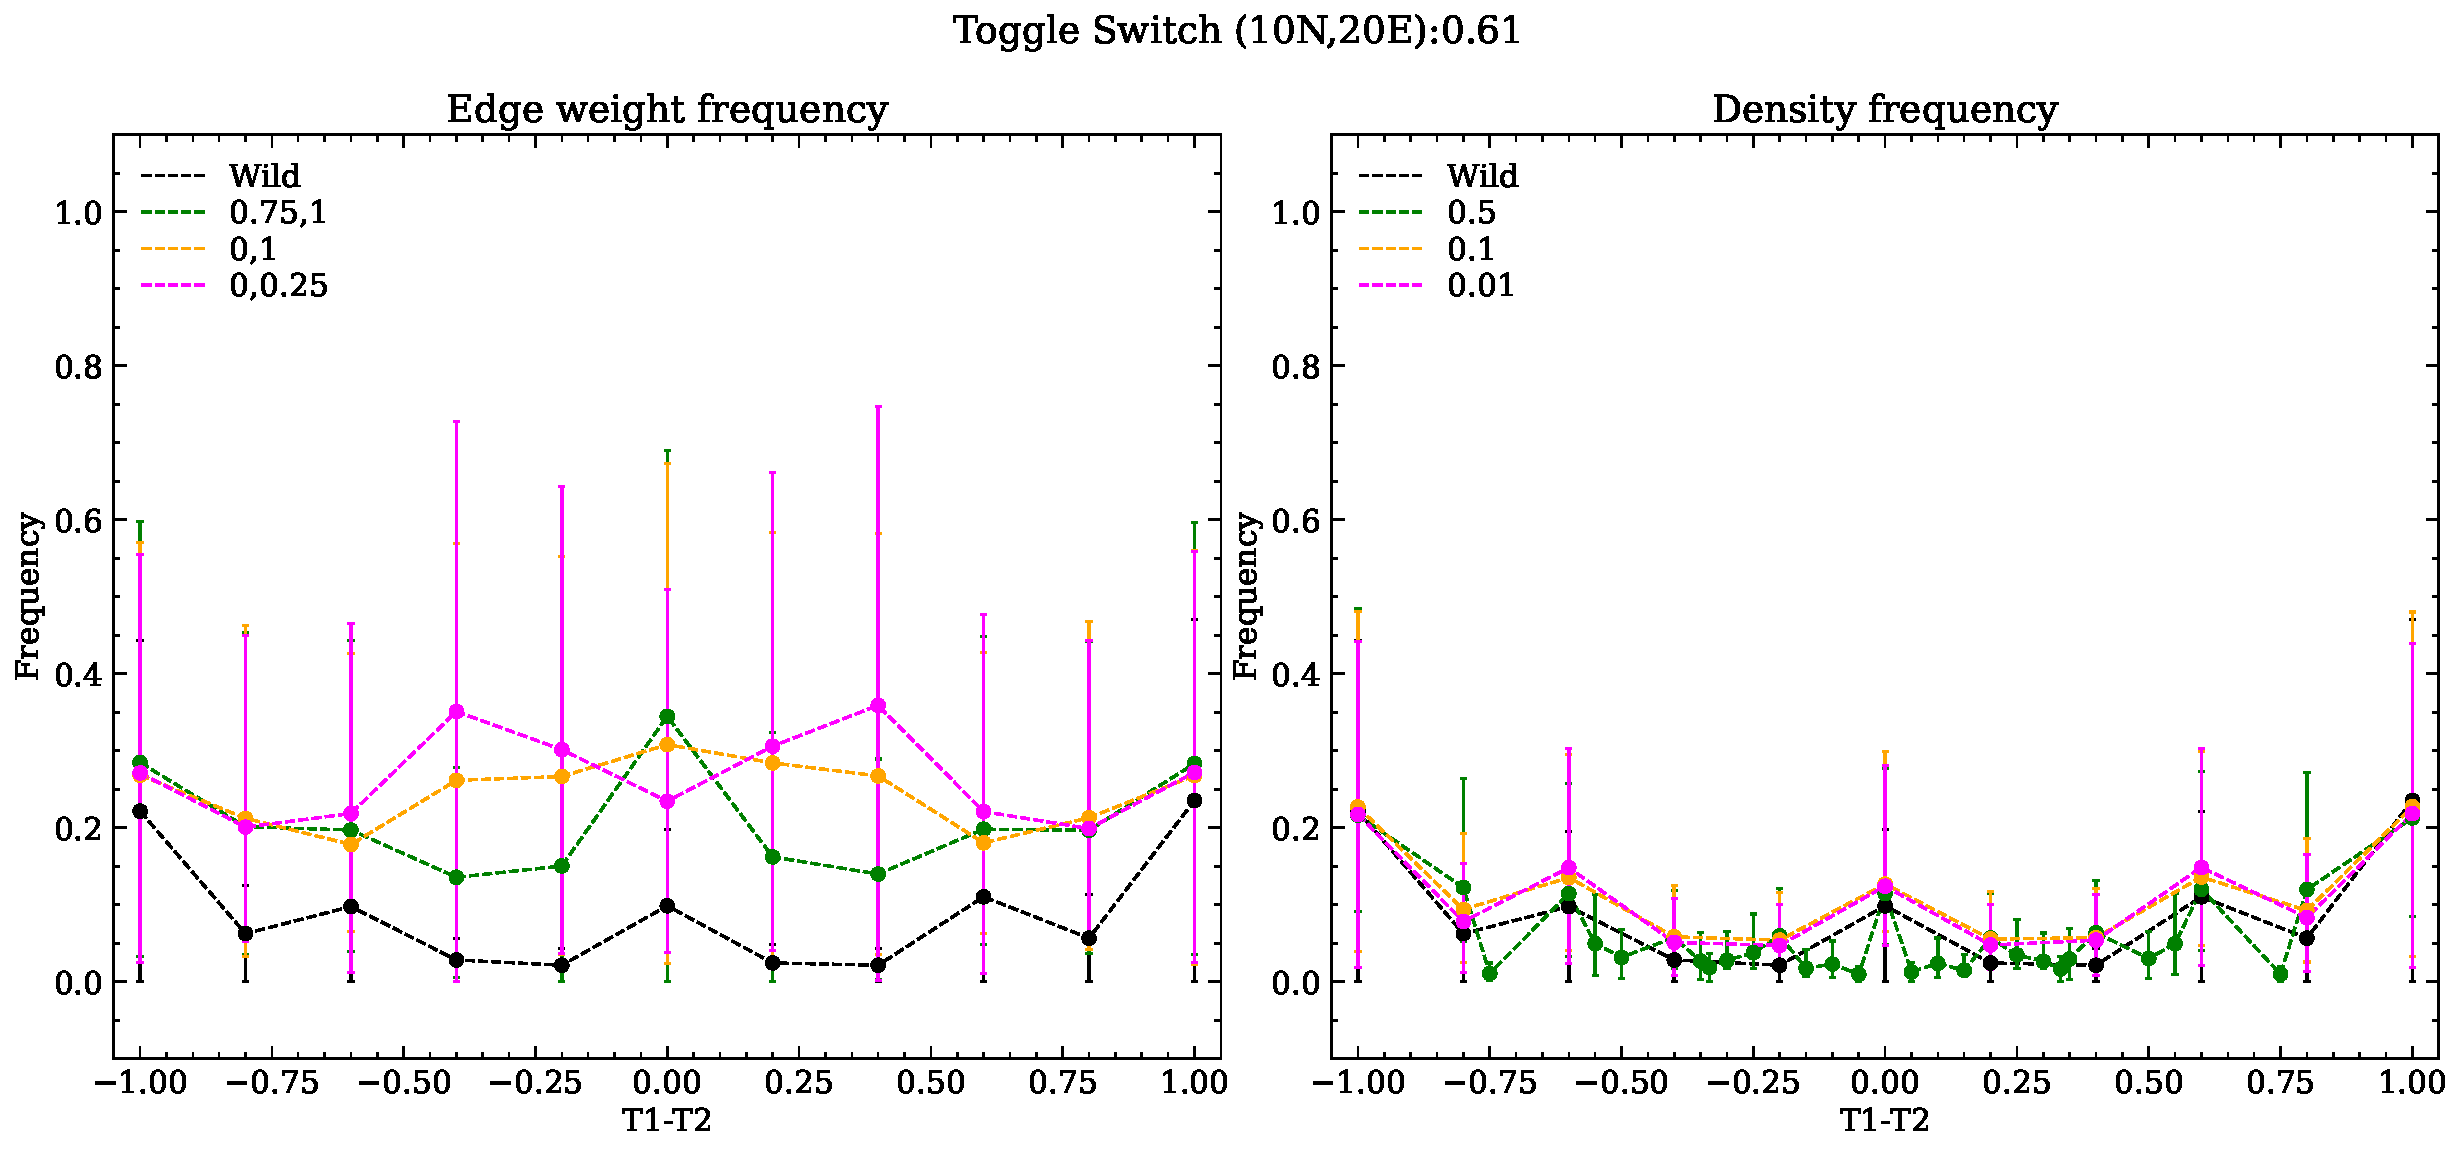
\includegraphics[height=0.3\textwidth,keepaspectratio]{Results/fig_1/fig1_ToggleSwitch_0.8.pdf} 
        \\[2pt]
        
        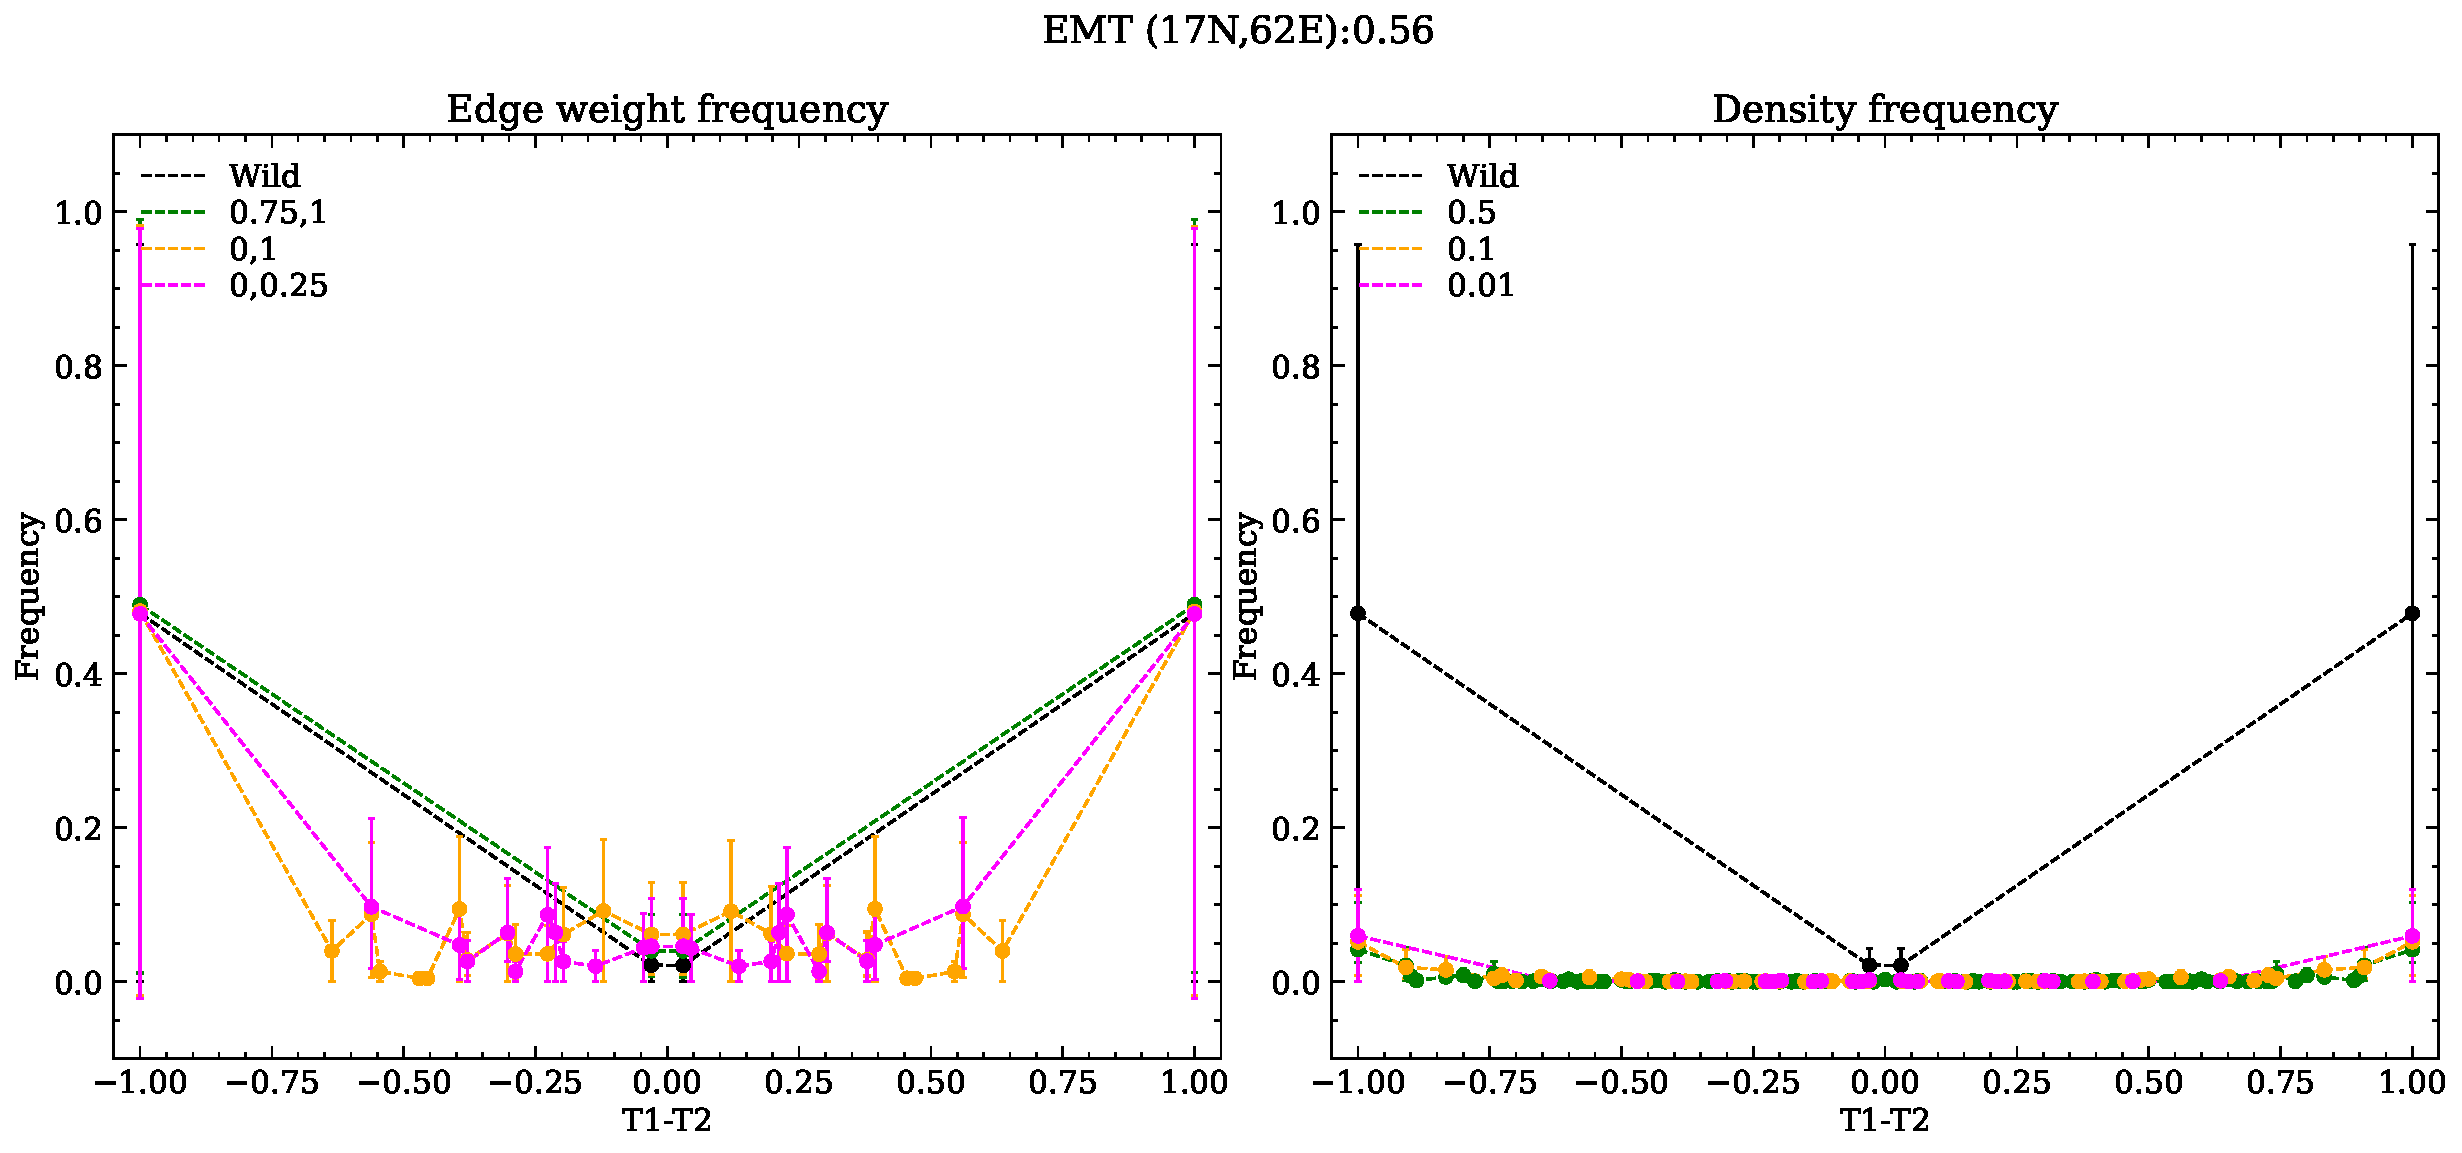
\includegraphics[height=0.3\textwidth]{Results/fig_1/fig1_EMT_RACIPE.pdf}\\
    \end{tabular} 
}
\caption{
\textbf{Steady-state frequencies of perturbed networks}: Steady-states are represented in terms of the difference in team expressions ($\mathrm{T1-T2}$) (x-axis);  The frequencies are for three levels of static perturbations (legend) to edge-weights (left) and density (right); The average frequencies (dots) and, the $25$-th (lower error bar) and the $75$-th (upper error bar) percentiles are displayed; The data in black belongs to the steady-state frequencies of the corresponding wild-type (unperturbed network); The top and bottom panels are of an artificial and a biological network, respectively; The titles in the panels display the network, the number of nodes and edges in the format ($x$N,$y$E) respectively, along with corresponding wild-type team strength (see Eq.~\ref{eq:ts_def}).
Generally, static perturbations negatively affect the dominant states of a network.
}
\label{fig:S1}
\end{figure*} 

\begin{figure*}
\setlength{\tabcolsep}{2pt}
\resizebox{1.05\textwidth}{!}{
\begin{tabular}{c c c c}

\textbf{(a)} &
{\hspace{-0.05cm}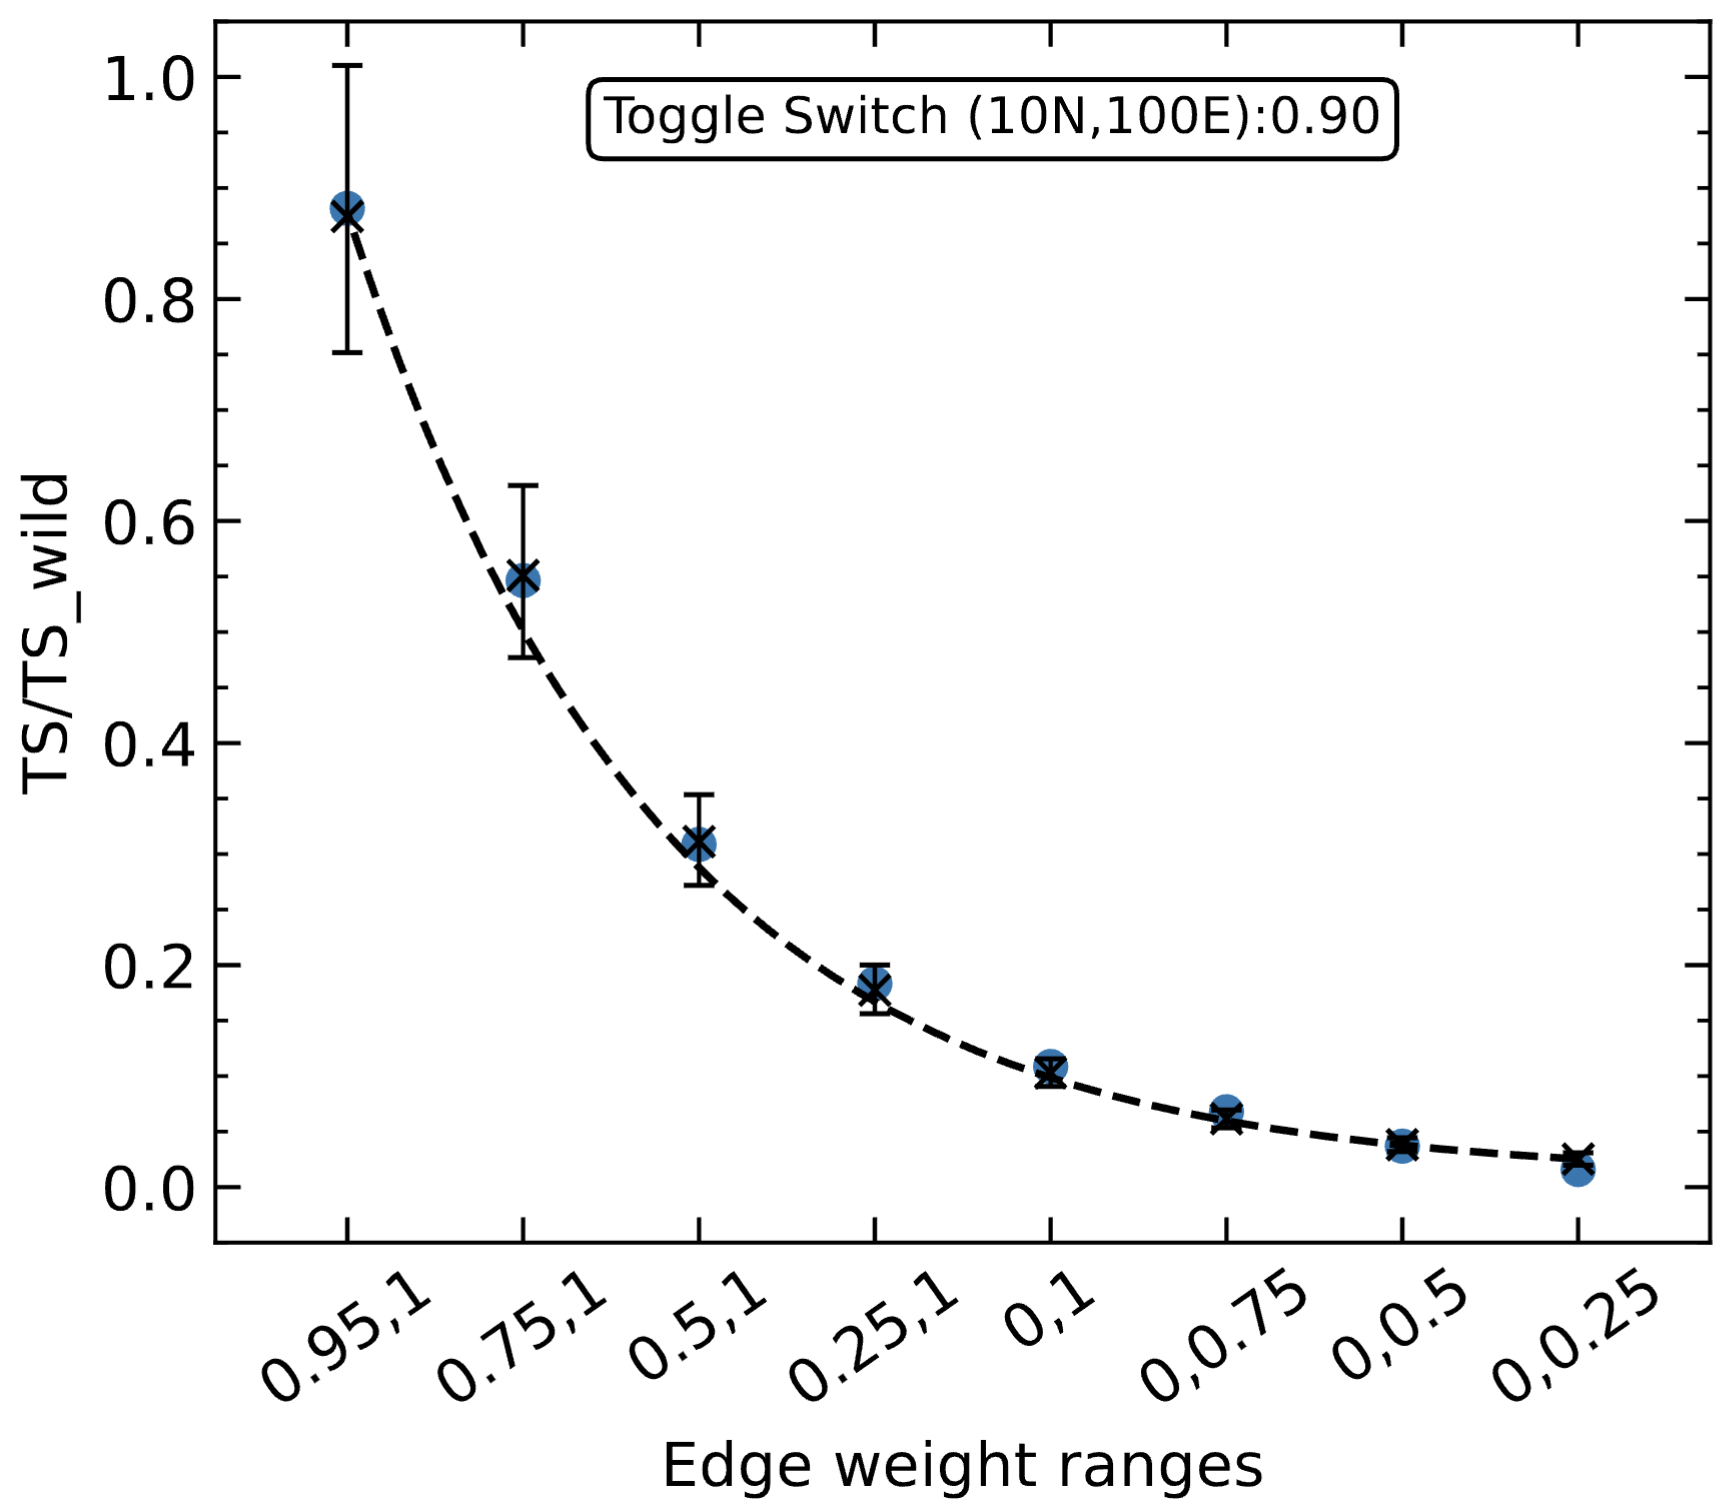
\includegraphics[width=2.83in,height=0.4\textwidth]{Results/ts_ew_ts.png}} &
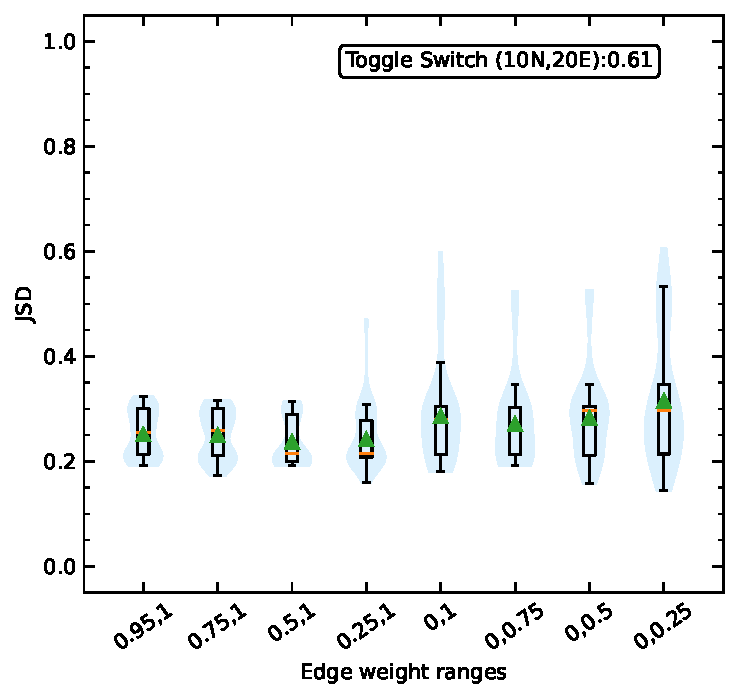
\includegraphics[width=2.85in,height=0.4\textwidth]{Results/JSD_compiled.pdf} &
\textbf{(b)} \\[2pt]

{\raisebox{0.8cm}{\hspace{-0.15cm}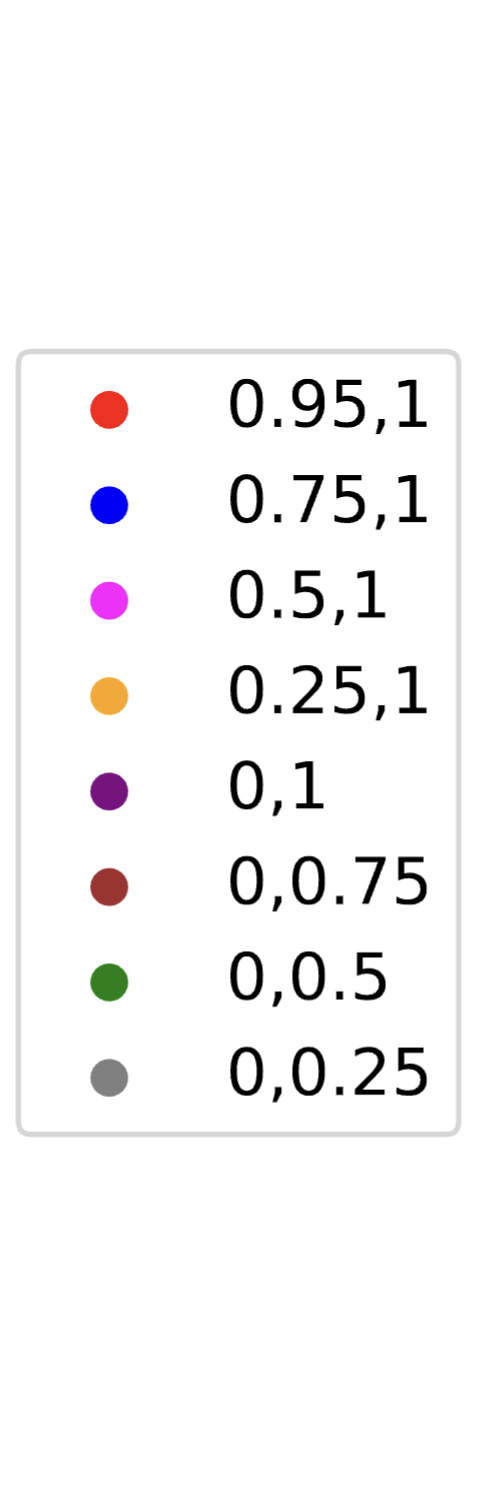
\includegraphics[height=0.3\textwidth,keepaspectratio]{Results/jsd_ts_net_ts.png}}} &
{\hspace{-0.15cm}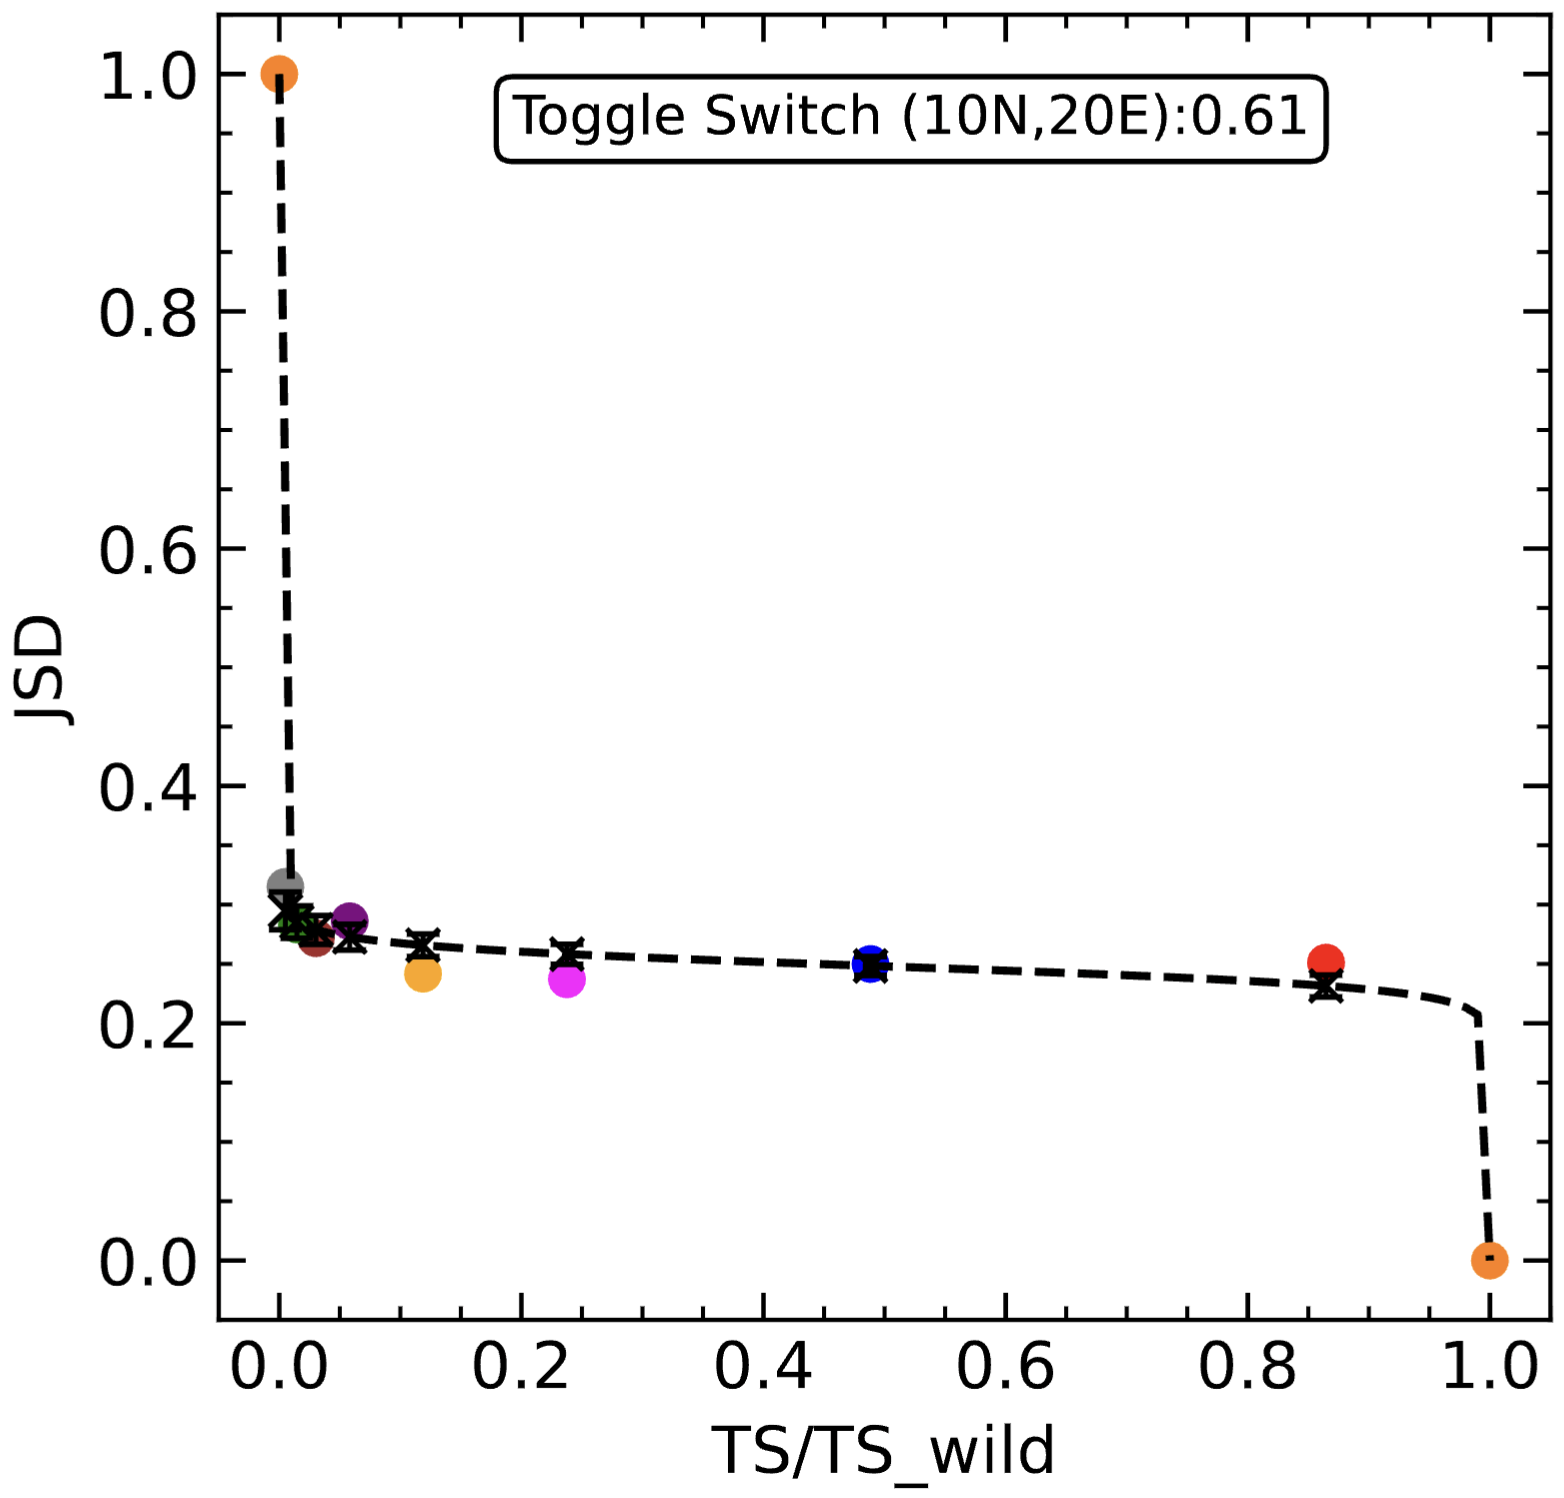
\includegraphics[width=2.9in,height=0.4\textwidth]{Results/jsd_ts_net_ts_fig.png}} &
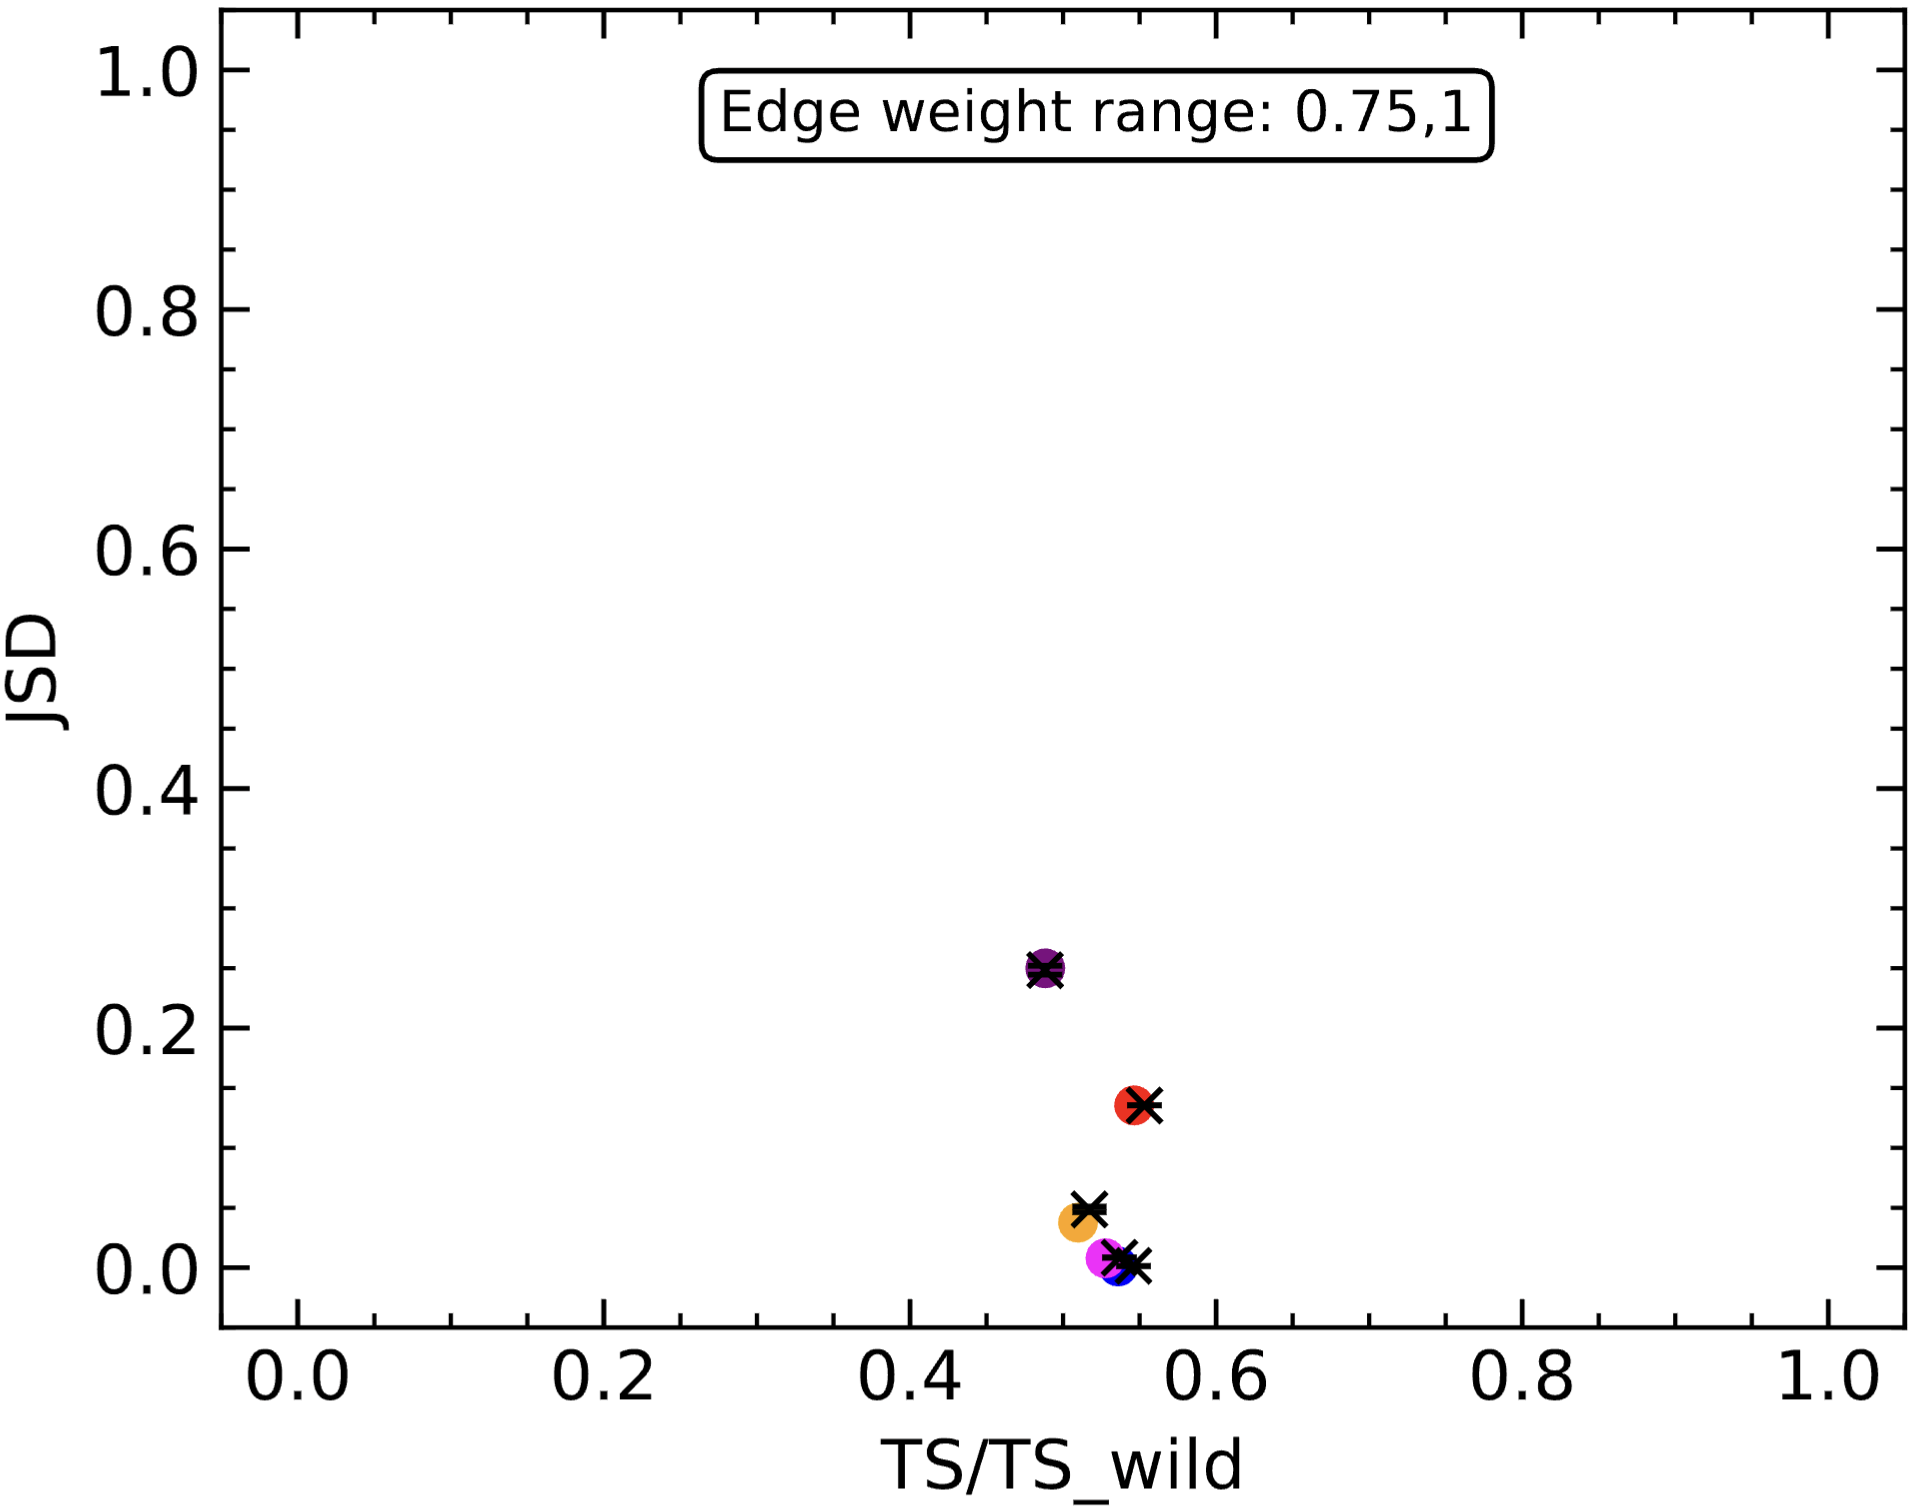
\includegraphics[height=0.4\textwidth]{Results/jsd_ts_ew_ts_fig.png} &
{\raisebox{0.8cm}{\hspace{-0.15cm}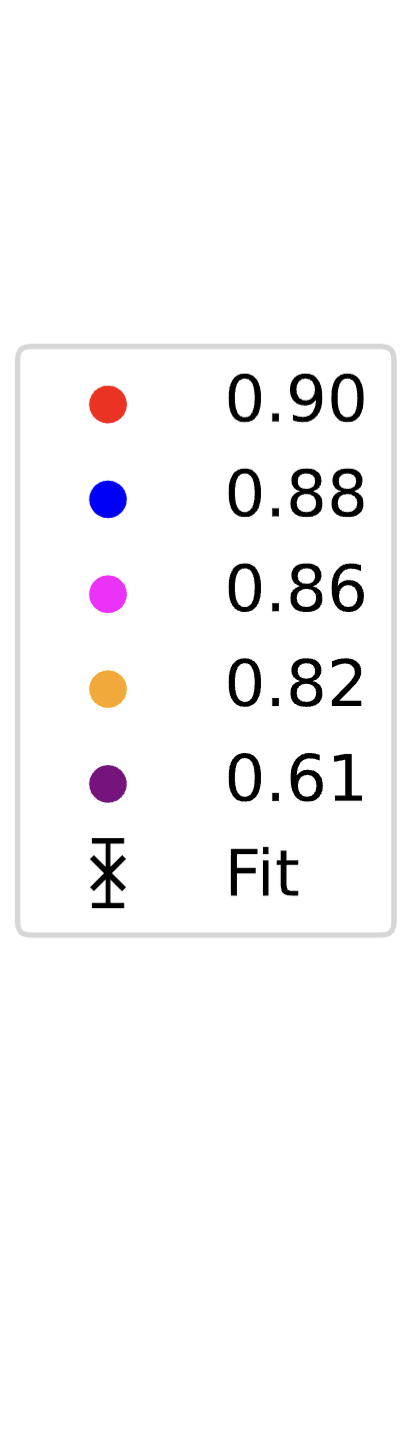
\includegraphics[height=0.3\textwidth]{Results/jsd_ts_ew_ts.png}}} \\[1.8pt]

{\raisebox{0.8cm}{\hspace{-0.15cm}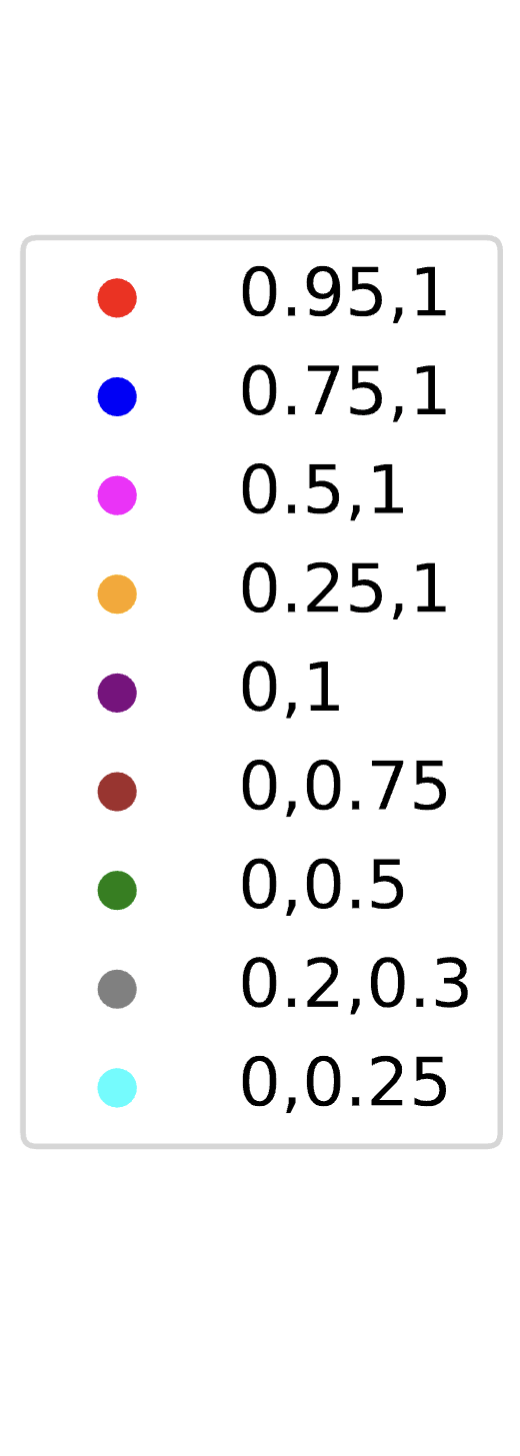
\includegraphics[height=0.3\textwidth,keepaspectratio]{Results/jsd_ts_net_bio.png}}} &
{\hspace{-0.05cm}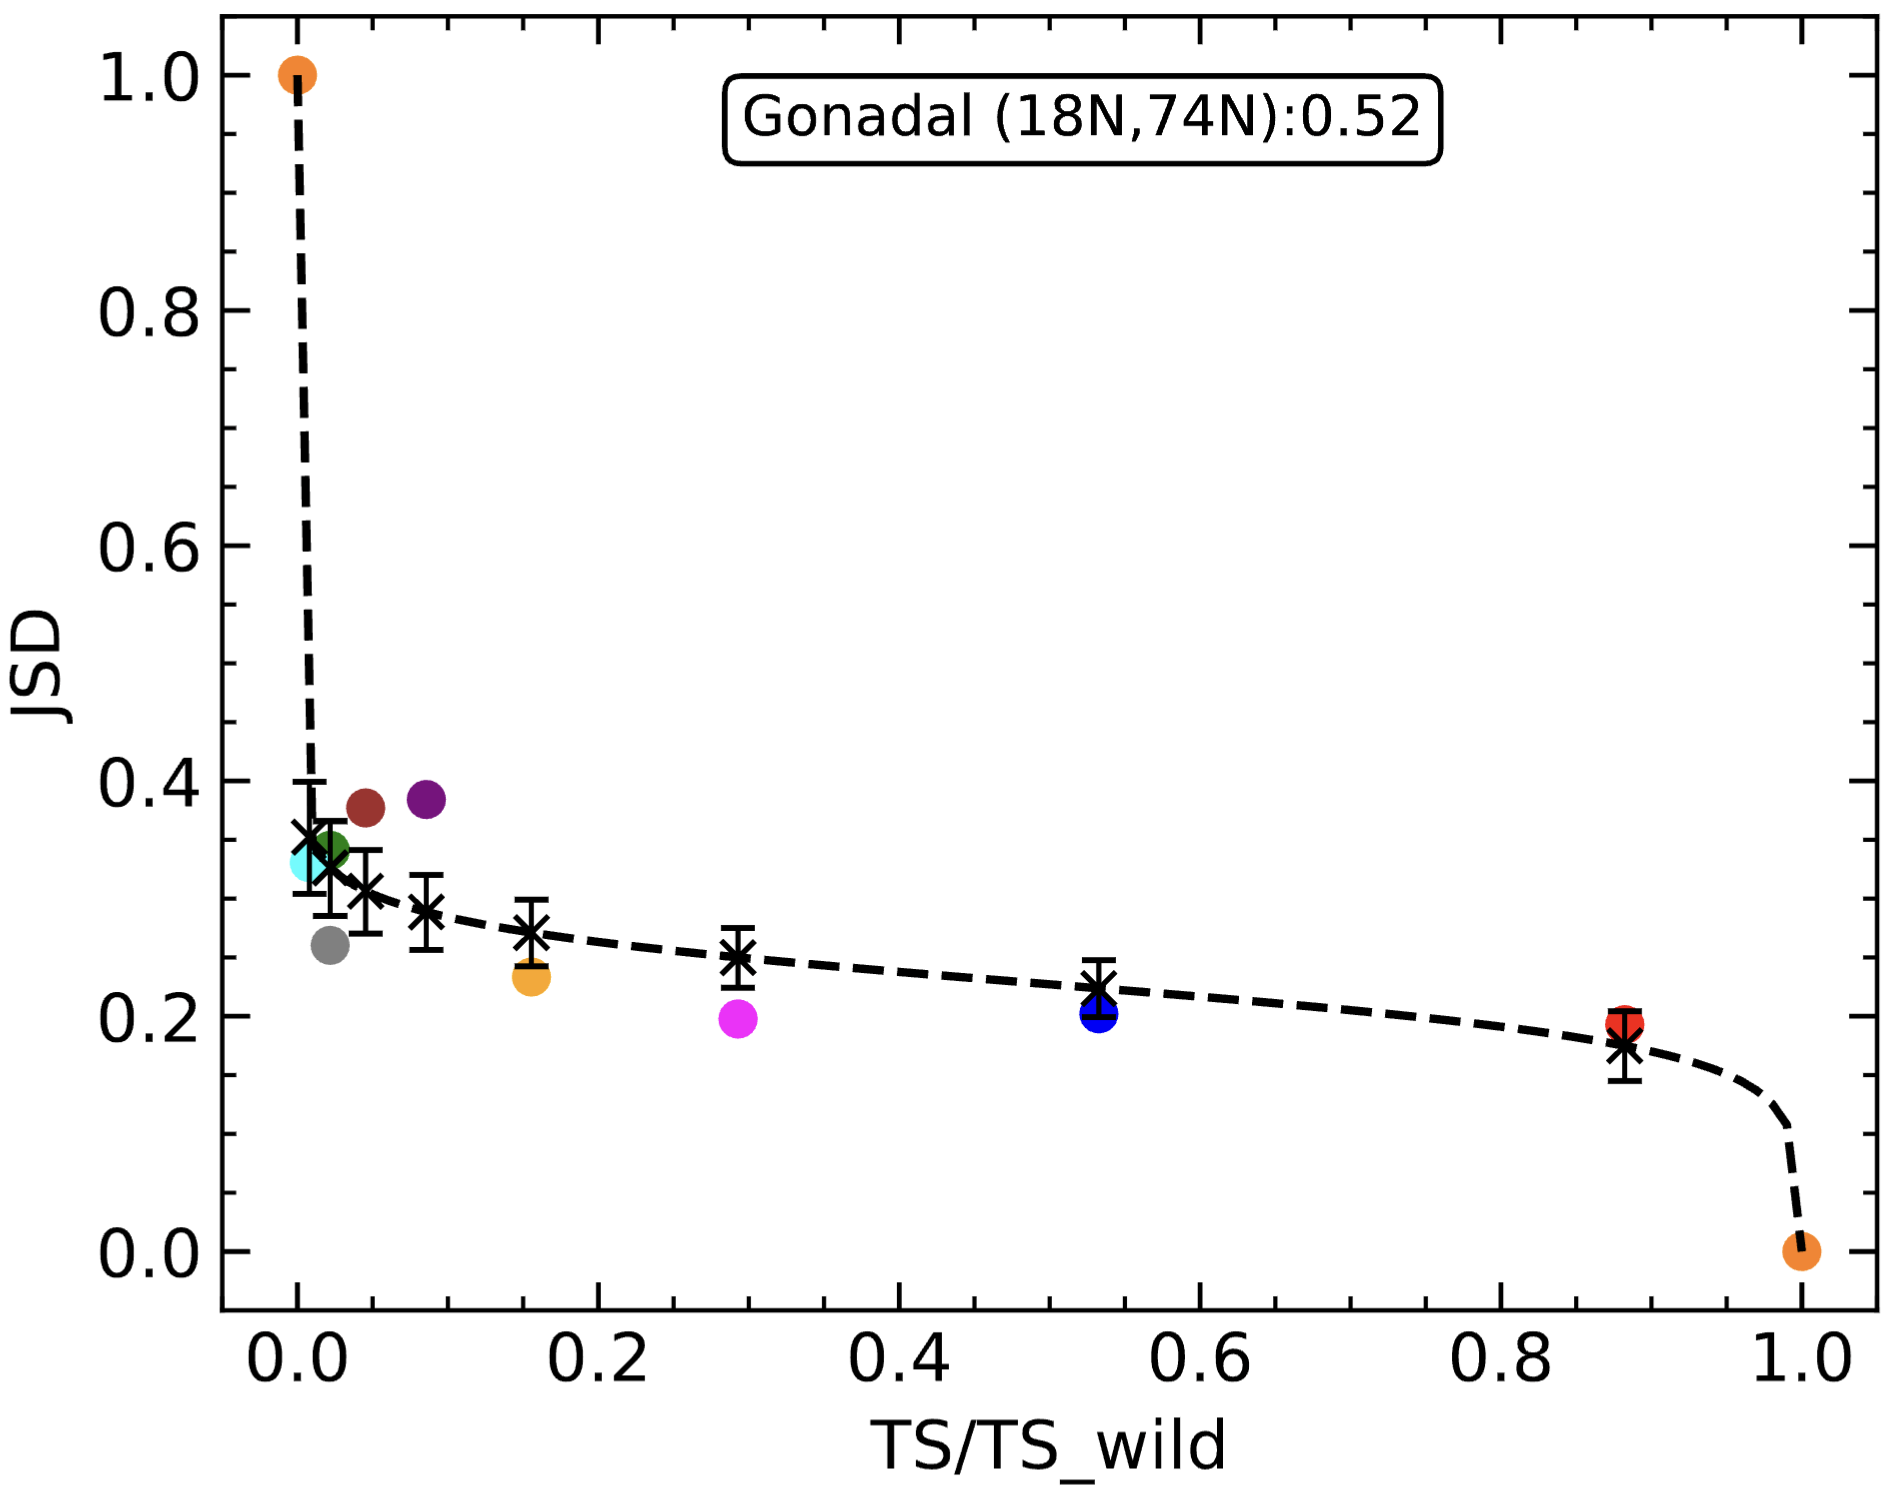
\includegraphics[height=0.4\textwidth]{Results/jsd_ts_net_bio_fig.png}} &
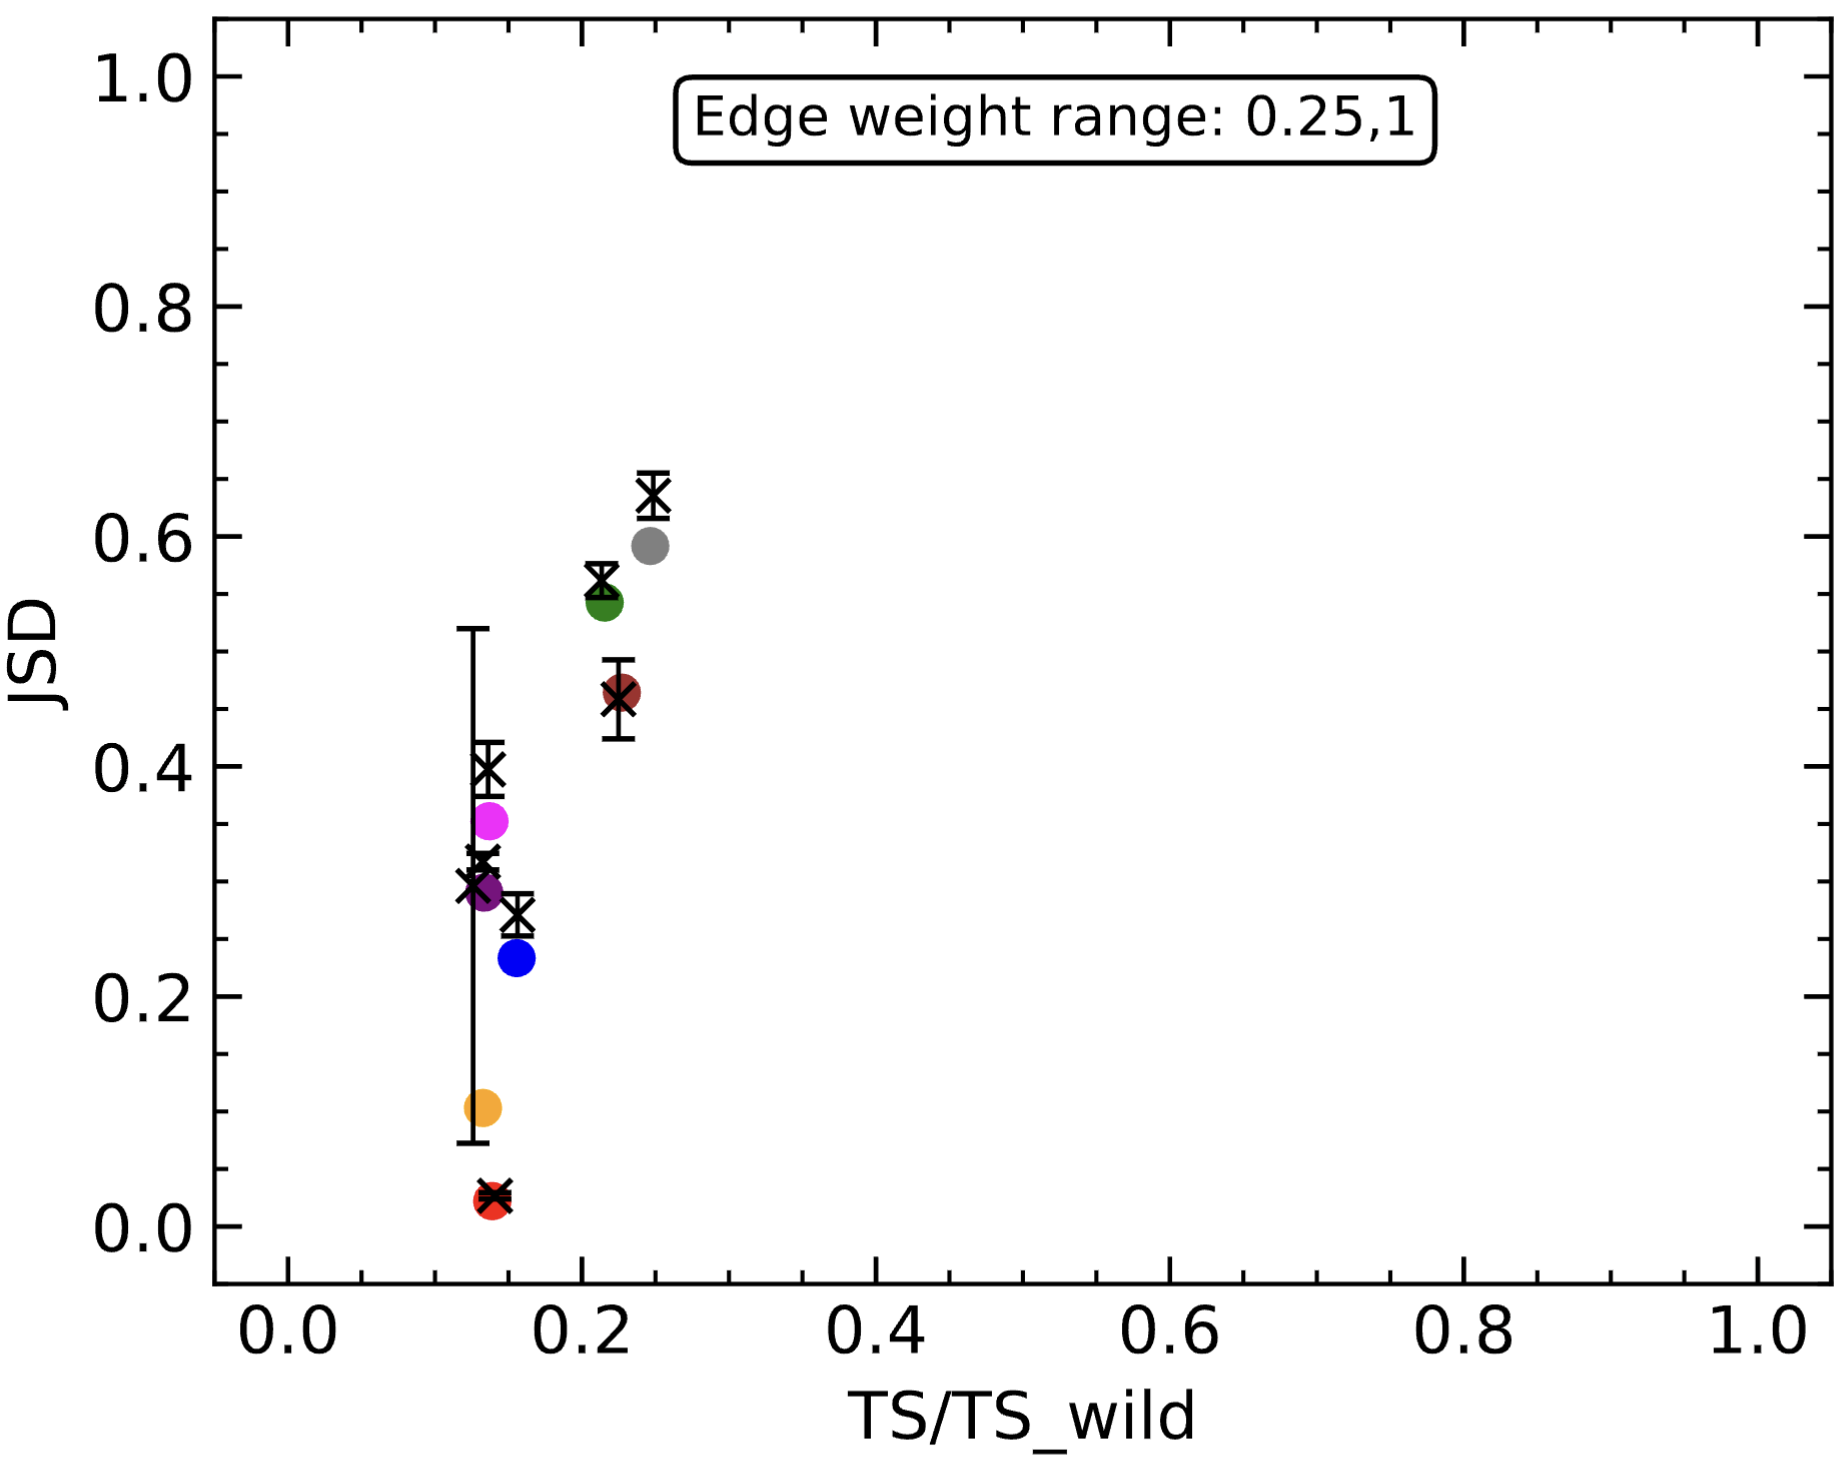
\includegraphics[height=0.4\textwidth]{Results/jsd_ts_ew_bio_fig.png} &
{\raisebox{0.8cm}{\hspace{-0.15cm}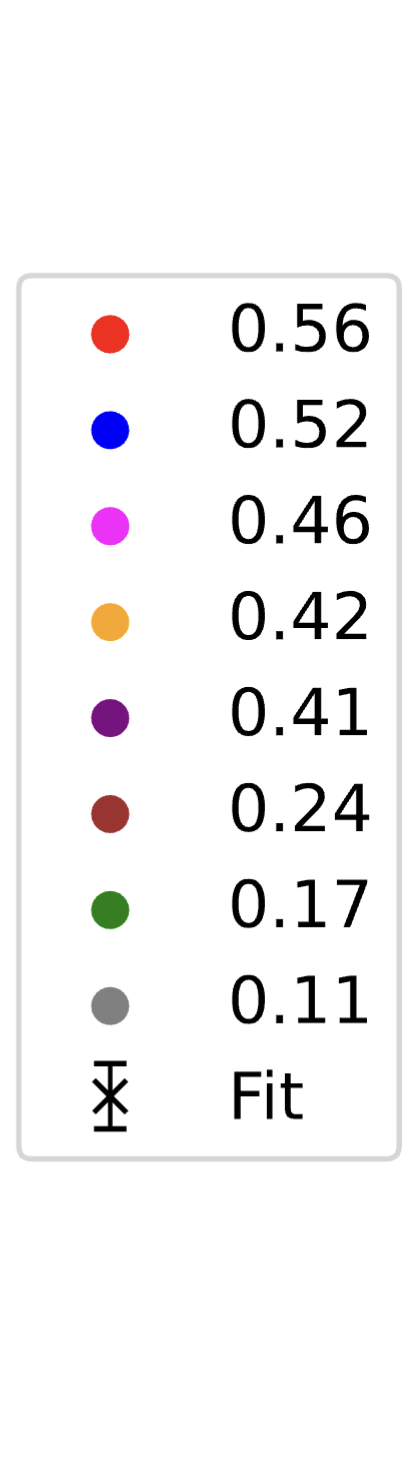
\includegraphics[height=0.3\textwidth]{Results/jsd_ts_ew_bio.png}}}

\end{tabular}
}
\caption{
\textbf{Quantification $\jsd$ as a function of $\ts/\tsw$ for static edge-weight perturbations}: Unless mentioned otherwise, the network along with its nodes, edges, and wild-type team strength is shown in the title. \textit{Top:} (right) Quantification of the mean of team-strength distributions ($\ts$) normalized by the corresponding wild-type team strength ($\tsw$), $\ts/\tsw$, as a function of the edge-weight noise levels ($\ewnum$; numerical values of the edge-weight noise ranges; see \S\ref{tt:ew_range_num}) using Eq.~\ref{eq:ts_ewnum} (black-dashed line) displayed along with the error bars (see Tab.~\ref{tab:ew_param}) for $\tsten$. (left) JSD distributions for edge-weight noise ranges along with their mean ($\jsd$) (green square) and median (orange line) for $\tseight$. \textit{Middle:} (right) Quantification $\jsd$ as a function of $\ts/\tsw$ for a given artificial network: Plot of $\jsd$ and $\ts/\tsw$ across edge-weight noise ranges (legend; left) along with their fit of the Eq.~\ref{eq:jsd_ts_net} (black-dashed line; see Tab.~\ref{tab:ew_param}) for $\tseight$; For an artificial network, the resilience of steady-state distribution increases with an increase in the strength of teaming interactions. (left) $\jsd$ vs. $\ts/\tsw$ for a given edge-weight noise level (in terms of range; here $[0.75,1]$; see title) across networks (represented in terms of their wild-type team strength $\tsw$; see legend); The data in black are $\jsd$ and their error bars obtained from Eq.~\ref{eq:jsd_ts_ran} with no fitting; For a static edge-weight noise level, the resilience increases with an increase in team strength across artificial networks. \textit{Bottom:} The plots represent the same as the middle panels except for biological networks. To rule out over-fitting, we have tested our models for the edge-weight noise range $[0.2,0.3]$ (see legend of left panel). The contrast is in the right panel where $\jsd$ increases with increasing $\ts/\tsw$; This observation remains to be explained.
}
\label{fig:S2}
\end{figure*} 

\newpage
% \section{Appendix}
\section{Distribution of $\lambda$ under additive noise}\label{AdditiveStationary}
\subsection*{Distribution of Additive noise $X \sim \mathrm{Uniform}[0,1]$, $Z \sim \mathcal{N}(0,\sigma^2)$}
\subsubsection{Notations}
\begin{align*}
    x => Current\ position \ of\ \lambda\\
    y => Next\ value\ of\ \lambda\\
    z = y-x \sim \mathcal{N}(0,\sigma^2)\\
    p(y\mid x) => Conditional\ probability\ of\ y\\
    p(y) => probability\ of\ y\\
    p_n(x) = \frac{1}{\sqrt{2\pi}\sigma}\exp^{\frac{-x^2}{2\sigma^2}}\\
    F_n(x_0) = p_n(x < x_0) = \int_{-\infty}^{x_0}p_n(x)dx
\end{align*}
%---------------------------------------------------------
\subsubsection*{Conditional distribution and continuous density}

For $y - x = z \sim \mathcal{N}(0,\sigma^2)$:
\begin{align*}
p(y \mid x) &= p_n(y - x)\big|_{0 < y < 1}
\end{align*}

\textbf{Point masses:}
\begin{align*}
p(y \mid x) &= p_n(k \leq -x)\big|_{y=0} \\
             &= p_n(k \geq 1 - x)\big|_{y=1}
\end{align*}

\textbf{Marginal density for $0 < y < 1$:}
% \begin{align*}
% p(y) &= p_n(y - x)\big|_{0 < y < 1} \\
%      &= F_n(-x)\big|_{y \leq 0} \\
%      &= 1 - F_n(1-x)\big|_{y \geq 1}
% \end{align*}

\begin{align*}
p(y)\big|_{0 < y < 1}
  &= \int_0^1 p(y \mid x)\,dx
   = \int_0^1 p_n(y-x)\,dx \\
  &= -\int_0^1 p_n(y-x)\,d(y-x) \\
  &= -\bigl[F_n(y-x)\bigr]_0^1 \\
\end{align*}

Hence: 
\begin{equation}
    p(y)\big|_{0 < y < 1} = F_n(y) - F_n(y-1)
\end{equation}
%---------------------------------------------------------
\subsubsection*{Point masses via integration by parts}

% \textbf{Aside:} The normal pdf and its CDF satisfy
% \[
%   \frac{1}{\sqrt{2\pi}\,\sigma}\,e^{-x^2/(2\sigma^2)}, \qquad
%   \frac{1}{\sqrt{2\pi}\,\sigma}, \qquad
%   p_n(0)\,e^{-1/(2\sigma^2)}
% \]

\textbf{Mass at $y = 0$:}
\begin{align*}
p(y=0)\big|_{y=0}
  &= \int_0^1 F_n(-x)\,dx
\end{align*}

\textbf{Mass at $y = 1$:}
\begin{align*}
p(y=1)\big|_{y=1}
  &= \int_0^1 \bigl(1 - F_n(1-x)\bigr)\,dx
\end{align*}

\textbf{Substitution} $u = 1-x$, $du = -dx$:
\begin{align*}
  &= -\int_1^0 \bigl(1 - F_n(u)\bigr)\,du
   = -\int_1^0 F_n(-u)\,du
   = \int_0^1 F_n(-u)\,du \\
  &= p(y=0)\big|_{y=1} \quad \Rightarrow \quad p(y=0) = p(y=1)
\end{align*}

\textbf{IBP:} $\int u\,dv = uv - \int v\,du$, with
$u = F_n(-x)$, $v = x$:
\[
  dv = dx, \qquad du = -p_n(-x)\,dx = -p_n(x)\,dx
\]

\textbf{Gaussian identity:}
\[
  x\,p_n(x) = -\sigma^2\,p_n'(x)
  \;\Longrightarrow\;
  x\,p_n(-x)\,dx = -\sigma^2\,d\,p_n(-x)
  \;\Longrightarrow\;
  x\,p_n(n)\,dx = -d\,p_n(\cdot)
\]

\begin{align*}
\int_0^1 F_n(-x)\,dx
  &= \bigl[x\,F_n(-x)\bigr]_0^1 + \int_0^1 x\,p_n(-x)\,dx \\
  &= F_n(-1) + \bigl[p_n(0) - p_n(1)\bigr] \cdot \sigma^2
\end{align*}

Hence:
\begin{equation}
    % \begin{align*}
    p(y=0) = p(y=1) = F_n(-1) + \sigma^2\bigl[p_n(0) - p_n(1)\bigr]
    % \end{align*}
\end{equation}


%---------------------------------------------------------
\subsubsection*{CDF for $0 \leq y_0 \leq 1$}

% \textbf{Summary so far:}
% \[
% \boxed{
% \begin{aligned}
% P(0) = P(1) &= F_n(-1) + \sigma^2\bigl[p_n(0) - p_n(1)\bigr] \\
% p(y)\big|_{0<y<1} &= F_n(y) - F_n(y-1)
% \end{aligned}
% }
% \]

Note: $F_n(x_0) = P_n(x \leq x_0)$.

\textbf{CDF:}
\begin{align*}
p(y < y_0)\\
  &= p(y = 0) + p(0 < y < y_0)\\
  &= F_n(-1) + \sigma^2\bigl[p_n(0) - p_n(1)\bigr]
   + \int_0^{y_0}\bigl(F_n(y) - F_n(y-1)\bigr)\,dy
\end{align*}

\textbf{Antiderivative of $F_n$} (IBP):
\begin{align*}
\int F_n(y)\,dy
  &= F_n(y)\cdot y - \int y\,p_n(y)\,dy \\
  &= F_n(y)\,y + \sigma^2\,p_n(y) + C
\end{align*}

\textbf{Definite integral:}
\begin{align*}
\int_0^{y_0} F_n(y)\,dy
  &= y_0\,F_n(y_0) + \sigma^2\bigl[p_n(y_0) - p_n(0)\bigr]
\end{align*}

\textbf{Shifted integral} via $u = y-1$, $du = dy$, $y=0 \Rightarrow u=-1$, $y=y_0 \Rightarrow u=y_0-1$:
\begin{align*}
\int_0^{y_0} F_n(y-1)\,dy
  &= \int_{-1}^{y_0-1} F_n(u)\,du
   = \int_{-1}^{0} F_n(u)\,du + \int_0^{y_0} F_n(u)\,du
\end{align*}

Therefore:
\begin{align}
p(y < y_0) &= p(0)
   - \int_{-1}^{y_0-1} F_n(y)\,dy
   + \int_0^{y_0} F_n(y)\,dy
\end{align}

%---------------------------------------------------------
\subsubsection*{Evaluating the CDF explicitly}

\[
\int F_n(y)\,dy = y\,F_n(y) + \sigma^2\,p_n(y) + C
\]

\begin{align*}
p(y \leq y_0)
  &= p(0)
   - \int_{-1}^{y_0-1} F_n(y)\,dy
   + \int_0^{y_0} F_n(y)\,dy \\[6pt]
  &= p(0)
   - \bigl[(y_0-1)\,F_n(y_0-1) - \sigma^2\,p_n(y_0-1)\bigr] \\
  &\quad - \bigl[(-1)\,F_n(-1) + \sigma^2\,p_n(-1)\bigr] \\
  &\quad + y_0\,F_n(y_0) + \sigma^2\,p_n(y_0) - \sigma^2\,p_n(0) \\[6pt]
  &= F_n(-1) + \sigma^2\bigl[p_n(0) - p_n(1)\bigr] \\
  &\quad - (y_0-1)\,F_n(y_0-1) - \sigma^2\,p_n(y_0-1) \\
  &\quad - F_n(-1) + \sigma^2\,p_n(-1) \\
  &\quad + y_0\,F_n(y_0) + \sigma^2\,p_n(y_0) - \sigma^2\,p_n(0) \\[6pt]
  &= y_0\,F_n(y_0) - (y_0-1)\,F_n(y_0-1)
   + \sigma^2\bigl[p_n(y_0) - p_n(y_0-1)\bigr] \\[6pt]
  &= y_0\,F_n(y_0) + (1-y_0)\bigl(1 - F_n(1-y_0)\bigr)
   + \sigma^2\bigl[p_n(y_0) - p_n(1-y_0)\bigr]
\end{align*}

%---------------------------------------------------------
\subsubsection*{Final form and complement}

\[
p(y \leq y_0)
  = y_0\,F_n(y_0)
  + (1-y_0)\bigl(1 - F_n(1-y_0)\bigr)
  + \sigma^2\bigl[p_n(y_0) - p_n(1-y_0)\bigr]
\]

\textbf{Complement $P(y_0 \leq Y \leq 1)$:}
\begin{align*}
p(y_0 \leq Y \leq 1)
  &= 1 - p(Y < y_0) \\
  &= 1 - \Bigl[
      y_0\,F_n(y_0)
      + (1-y_0)\bigl(1-F_n(1-y_0)\bigr)
      + \sigma^2\bigl[p_n(y_0) - p_n(1-y_0)\bigr]
    \Bigr]
\end{align*}

\textbf{Substitution} $y_0 = 1 - y'$:
\begin{align*}
  &= 1 - \Bigl[
      (1-y')\,F_n(1-y')
      + y'\bigl(1 - F_n(y')\bigr)
      + \sigma^2\bigl[p_n(1-y') - p_n(y')\bigr]
    \Bigr] \\[4pt]
  &= 1 - (1-y')\,F_n(1-y') - y' + y'\,F_n(y') \\
  &\quad - \sigma^2\,p_n(1-y') + \sigma^2\,p_n(y') \\[4pt]
  &= (1-y')\bigl(1 - F_n(1-y')\bigr)
   + y'\,F_n(y')
   + \sigma^2\bigl[p_n(y') - p_n(1-y')\bigr]
\end{align*}

%---------------------------------------------------------
\subsubsection*{Summary and numerical example}

\[
\boxed{
\begin{aligned}
p(0) = p(1)
  &= F_n(-1) + \sigma^2\bigl[p_n(0) - p_n(1)\bigr] \\
p(y)\big|_{0<y<1}
  &= F_n(y) - F_n(y-1)
\end{aligned}
}
\]

\begin{equation}
p(y \leq y_0)
  = y_0\,F_n(y_0)
  + (1-y_0)\bigl(1 - F_n(1-y_0)\bigr)
  + \sigma^2\bigl[p_n(y_0) - p_n(1-y_0)\bigr]
  \label{additiveCDF}
\end{equation}

\textbf{Note:} this also equals $p(y_0 \leq Y \leq 1)$ by symmetry. \\[6pt]

% We find a reasonable strong agreement between the simuated and analytically derived distributions, as shown below. 

% \begin{figure}
%     \centering
%     
\includegraphics[width=\linewidth]{AditiveNoiseFigures/prob_dist_compare.jpg}
%     \caption{\textbf{Comparision of CDFs generated from simulations and the analytical calculations} Each panel shows the cumulative distribution obtained from Eq \ref{additiveCDF} (red) and numerically calculated trajectories (green). The CDFs agree well with each other, with minor differences that should not have any strong impact on sampling lambda values.} 
%     \label{fig:noiseDist}
% \end{figure}


\section{Evaluating the effect of additive noise against the corresponding stationary distribution}

Additive noise leads to an increase in node expression, increasing the residence time of hybrid states ((1,1) state in toggle switch). Among the three noises tested, additive noise also has the highest variance, with a high chance of achieving $\lambda \approx 1$ - weakening the inhibitions in the toggle switch and potentially allowing the nodes to express independently. Thus, it is important to understand if increasing hybrid state MRT is due to the distribution of $\lambda$s created by the additive noise or if the noise itself is required. We thus perfomed experiments to answer the following questions

\begin{enumerate}

    \item Do deterministic simulations of the toggle switch parameters with $\lambda$ sampled from the distributions generated by additive noise lead to an increase in the MRT of (1, 1) state?
    \item Does modifying the noise to ensure lambda switching between 0.01 and 1 (instead of increments by normal random variable) increase the frequency of the (1, 1) state?
\end{enumerate}
The original formulation of additive noise follows the equation below:

\begin{equation}
\begin{split}
    \lambda(t+1) &\overset{\text{Additive}}{=} 
        \lambda(t) + \mathcal{N}(0,\sigma)\\
    \lambda(t+1) &= \text{clip}\bigl(\lambda(t+1),\ 0.01,\ 1\bigr)
\end{split}
\label{additiveNoise}
\end{equation}

We devised two additional forms of noise - named the Jumping noise and the Extreme noise - defined as follows:


% \centering
\begin{equation}
\begin{split}
    \lambda(t+1) &\overset{\text{Jumping}}{=} 
    \begin{cases}
        \lambda(t) + \sigma & \text{if } \mathcal{N}(0,\sigma) > 0 \\
        \lambda(t) - \sigma & \text{if } \mathcal{N}(0,\sigma) < 0
    \end{cases} \\[6pt]
    \lambda(t+1) &= \text{clip}\bigl(\lambda(t+1),\ 0.01,\ 1\bigr)
\end{split}
\label{jumpingNoise}
\end{equation}

\begin{equation}
    \lambda (t+1) \overset{Extreme}{=} \begin{cases}
        1 \ if \ N(0,\sigma) > 0\\
        0.01 \ if \ N(0,\sigma) < 0
    \end{cases}
    \label{extremeNoise}
\end{equation}



We then derived the distribution of $\lambda$ for five values of $\sigma$ : ${0.001, 0.005, 0.01, 0.05, 0.1}$ numerically and simulated toggle switch as follows:

\begin{itemize}
    \item Sample a subset of models $\{m_i\}$ from RACIPE and extract the $\lambda$ values
    \item For each such $\lambda$, run 100 trajectories of $\lambda$, using the corresponding noise equation (Eq \ref{additiveNoise}, \ref{jumpingNoise}, \ref{extremeNoise}), for 10000 time steps.
    \item Collect the values of $\lambda$ from all the 100 trajectories to use as the distribution for the corresponding noise type. 
    \item Generate 10 new models $\{m_{i_j}\}$, each model having the same parameters as the original RACIPE model, except for the $\lambda$ values sampled from the distribution generated in the previous step.
    \item Generate deterministic trajectories for each model starting from 100 randomly generated initial conditions sampled uniformly from the range $[0, \frac{g_A}{k_A}]$, where $g_A$ is the production rate of node $A$ and $k_A$ is the degradation rate. Run each simulation for 10000 time steps
    \item Discretize each state along these simulations using the threshold values obtained from RACIPE. 
    \item Evaluate the mean fraction of occurence of each discrete state across all simulations and the 10 models.
    \item Parallely run stochastic simulations on the original models of RACIPE $\{m_i\}$, starting from the steady states obtained from RACIPE, with $\lambda$ being updated at each time point according to Eq \ref{additiveNoise}, \ref{jumpingNoise}, \ref{extremeNoise}. Evaluate mean residence times of the discrete states across these stochastic trajectories.
\end{itemize}

\subsection{Comparing the MRTs of stochastic and deterministic trajectories}

\begin{figure}
    \centering
    \begin{subfigure}[t]{0.48\linewidth}
        
\includegraphics[width=\linewidth]{AditiveNoiseFigures/11Additive.jpg}
        \caption{Additive noise}
        \label{fig:additive11}
    \end{subfigure}
    \hfill
    \begin{subfigure}[t]{0.48\linewidth}
        
\includegraphics[width=\linewidth]{AditiveNoiseFigures/11Jumping.jpg}
        \caption{Jumping noise}
        \label{fig:jumping11}
    \end{subfigure}

    \begin{subfigure}[t]{0.48\linewidth}
        
\includegraphics[width=\linewidth]{AditiveNoiseFigures/11Extreme.jpg}
        \caption{Extreme noise}
        \label{fig:extreme11}
    \end{subfigure}
    \caption{Boxplots showing the comparison of MRTs of the (1,1) state from deterministic (red) and stochastic (green) simulations of Additive, Jumping and Extreme noise. The mean of the each distribution is shown using a '+' symbol, while the median is shown by a black horizontal line segment within each box. The boundaries of the boxes show the IQR.}
    \label{fig:11MRT}
\end{figure}

For both additive and jumping noise, the mean MRT of the (1,1) state is nearly the same for both stochastic and deterministic simulations. Two differences can be highlighted: (1) the median MRT is either 0 or 1 in deterministic simulations irrespective of $\sigma$, whereas the corresponding median for stochastic simulations increases with $\sigma$. (2) The overall distribution for deterministic simulations is extremely bimodal, whereas that for the stochastic simulations shifts to higher values with increasing $\sigma$. These observations suggest that the distribution alone can indeed increase the incidence of (1,1) state in additive noise, but the increase is not consistent. The stochasticity ensures that the MRT of (1,1) remains high. Similar observations can be seen for the jumping noise case. Interestingly, in the case of extreme noise where the $\lambda$ can either be high (1) or low (0.01), the mean MRT in deterministic simulations is always lower than that of stochastic simulations, which could be explained by the fact that given only 4 combinations of $\lambda$ are possible, only one of the combinations can reliably allow the stability of (1,1) state - where both $\lambda$ values are 1. 

\begin{figure}
    \centering
    \begin{subfigure}[t]{0.48\linewidth}
        
\includegraphics[width=\linewidth]{AditiveNoiseFigures/01Additive.jpg}
        \caption{Additive noise}
        \label{fig:additive01}
    \end{subfigure}
    \hfill
    \begin{subfigure}[t]{0.48\linewidth}
        
\includegraphics[width=\linewidth]{AditiveNoiseFigures/01Jumping.jpg}
        \caption{Jumping noise}
        \label{fig:jumping01}
    \end{subfigure}

    \begin{subfigure}[t]{0.48\linewidth}
        
\includegraphics[width=\linewidth]{AditiveNoiseFigures/01Extreme.jpg}
        \caption{Extreme noise}
        \label{fig:extreme01}
    \end{subfigure}
    \caption{Boxplots showing the comparison of MRTs of the (0,1) state from deterministic (red) and stochastic (green) simulations of Additive, Jumping and Extreme noise. The mean of the each distribution is shown using a '+' symbol, while the median is shown by a black horizontal line segment within each box. The boundaries of the boxes show the IQR.}
    \label{fig:01MRT}
\end{figure}

\section{Distribution of $\lambda$ under multiplicative noise}
\label{MultiplicativeStationary}

\subsection*{Distribution under Multiplicative Noise:
  $X \sim \mathrm{Uniform}[0,1]$, $Y = X(1 + Z)$, $Z \sim \mathcal{N}(0,\sigma^2)$}

\subsubsection*{Notation}
\begin{align*}
  x &\Rightarrow \text{current position of } \lambda \\
  y &\Rightarrow \text{next value of } \lambda \\
  z &= \frac{y}{x} - 1 \sim \mathcal{N}(0,\sigma^2) \\
  p(y \mid x) &\Rightarrow \text{conditional probability of } y \\
  p(y) &\Rightarrow \text{marginal probability of } y \\
  p_n(x) &= \frac{1}{\sqrt{2\pi}\,\sigma}
            \exp\!\left(-\frac{x^2}{2\sigma^2}\right) \\
  F_n(x_0) &= P(x \leq x_0) = \int_{-\infty}^{x_0} p_n(x)\,dx
\end{align*}

We also define the auxiliary function
\begin{equation}
  g(a) \;=\; \int_a^{\infty} \frac{p_n(t)}{1+t}\,dt,
  \label{eq:gdef}
\end{equation}
which will appear throughout. Note $g'(a) = -p_n(a)/(1+a)$.

%---------------------------------------------------------
\subsubsection*{Conditional distribution given $X = x$}

Since $Y = x(1+Z)$ and the state space is clamped to $[0,1]$:
\begin{itemize}
  \item $Y = 0$ iff $x(1+Z) \leq 0$, i.e.\ $Z \leq -1$ (for $x > 0$),
  \item $Y = 1$ iff $x(1+Z) \geq 1$, i.e.\ $Z \geq 1/x - 1$,
  \item $Y = y \in (0,1)$ otherwise, with $z = y/x - 1$.
\end{itemize}

Applying the change-of-variables $z = y/x - 1$, $dz = dy/x$:

\begin{equation}
  p(y \mid x) = \begin{cases}
    F_n(-1) & y = 0 \\[4pt]
    \dfrac{1}{x}\,p_n\!\left(\dfrac{y}{x} - 1\right) & 0 < y < 1 \\[8pt]
    1 - F_n\!\left(\dfrac{1}{x} - 1\right) & y = 1
  \end{cases}
  \label{eq:conditional_mult}
\end{equation}

%---------------------------------------------------------
\subsubsection*{Point mass at $y = 0$}

The boundary condition $Y = 0$ requires $Z \leq -1$, independently of $x$:
\begin{align*}
  p(y = 0)
    &= \int_0^1 P(Y=0 \mid X=x)\,dx
     = \int_0^1 F_n(-1)\,dx
\end{align*}
\begin{equation}
  \boxed{p(y=0) = F_n(-1)}
  \label{eq:mass0_mult}
\end{equation}

\textbf{Note:} Unlike the additive case, $p(y=0)$ depends only on $\sigma$
and not on the position $x$, because the sign change requires $Z < -1$
regardless of $x$.

%---------------------------------------------------------
\subsubsection*{Point mass at $y = 1$}

\begin{align*}
  p(y=1)
    &= \int_0^1 \left[1 - F_n\!\left(\tfrac{1}{x}-1\right)\right] dx
\end{align*}

\textbf{Substitution} $u = 1/x - 1$, so $x = 1/(1+u)$,
$dx = -du/(1+u)^2$; $x=1 \Rightarrow u=0$, $x \to 0^+ \Rightarrow u \to \infty$:

\begin{align*}
  p(y=1)
    &= \int_0^{\infty} \frac{1-F_n(u)}{(1+u)^2}\,du
\end{align*}

\textbf{IBP} with $A = 1-F_n(u)$, $dB = (1+u)^{-2}\,du$,
so $B = -(1+u)^{-1}$:

\begin{align*}
  &= \left[-\frac{1-F_n(u)}{1+u}\right]_0^{\infty}
     - \int_0^{\infty} \frac{p_n(u)}{1+u}\,du \\
  &= \left(0 - \frac{1-F_n(0)}{1}\right) - g(0) \\
  &= \frac{1}{2} - g(0)
\end{align*}

\begin{equation}
  \boxed{p(y=1) = \tfrac{1}{2} - g(0)}
  \label{eq:mass1_mult}
\end{equation}

\textbf{Note:} $p(y=0) \neq p(y=1)$ in general; the symmetry of the additive
case is broken because multiplicative noise scales with position.

%---------------------------------------------------------
\subsubsection*{Continuous density for $0 < y < 1$}

\begin{align*}
  p(y)
    &= \int_0^1 \frac{1}{x}\,p_n\!\left(\frac{y}{x}-1\right)dx
\end{align*}

\textbf{Substitution} $t = y/x - 1$, so $x = y/(1+t)$,
$dx = -y/(1+t)^2\,dt$; $x=1 \Rightarrow t=y-1$,
$x \to 0^+ \Rightarrow t \to \infty$:

\begin{align*}
  p(y)
    &= \int_{y-1}^{\infty}
       \frac{1+t}{y}\,p_n(t)\cdot\frac{y}{(1+t)^2}\,dt
     = \int_{y-1}^{\infty} \frac{p_n(t)}{1+t}\,dt
\end{align*}

\begin{equation}
  \boxed{p(y) = g(y-1), \qquad 0 < y < 1}
  \label{eq:density_mult}
\end{equation}

where $g$ is defined in Eq.~\eqref{eq:gdef}.
Note that for $y \in (0,1)$ the lower limit $y-1 \in (-1,0)$, so the
integral is always well-defined. 

%---------------------------------------------------------
\subsubsection*{CDF for $0 \leq y_0 \leq 1$}

\begin{align*}
  P(Y \leq y_0)
    &= p(y=0) + \int_0^{y_0} p(y)\,dy \\
    &= F_n(-1) + \int_0^{y_0} g(y-1)\,dy
\end{align*}

\textbf{Substitution} $s = y-1$, $ds = dy$:
\begin{align*}
  \int_0^{y_0} g(y-1)\,dy
    &= \int_{-1}^{y_0-1} g(s)\,ds
\end{align*}

\textbf{Switching order of integration} (Fubini) in
$\int_{-1}^{y_0-1} \int_s^{\infty} \frac{p_n(t)}{1+t}\,dt\,ds$:

\begin{align*}
  &= \int_{-1}^{\infty} \frac{p_n(t)}{1+t}
     \int_{-1}^{\min(t,\,y_0-1)} ds\,dt \\[4pt]
  &= \int_{y_0-1}^{\infty} \frac{p_n(t)}{1+t}\cdot y_0\,dt
   + \int_{-1}^{y_0-1} \frac{p_n(t)}{1+t}\cdot(t+1)\,dt \\[4pt]
  &= y_0\,g(y_0-1)
   + \int_{-1}^{y_0-1} p_n(t)\,dt \\[4pt]
  &= y_0\,g(y_0-1) + F_n(y_0-1) - F_n(-1)
\end{align*}

Therefore:
\begin{equation}
  \boxed{P(Y \leq y_0)
    = y_0\,g(y_0 - 1) + F_n(y_0 - 1)}
  \label{eq:CDF_mult}
\end{equation}

%---------------------------------------------------------
\subsubsection*{Sanity checks}

\textbf{At $y_0 = 0$:}
\[
  P(Y \leq 0) = 0 \cdot g(-1) + F_n(-1) = F_n(-1) = p(y=0) \;\checkmark
\]

\textbf{At $y_0 = 1$:}
\begin{align*}
  P(Y < 1) &= g(0) + F_n(0) = g(0) + \tfrac{1}{2} \\
  P(Y \leq 1) &= P(Y < 1) + p(y=1)
               = g(0) + \tfrac{1}{2} + \tfrac{1}{2} - g(0) = 1 \;\checkmark
\end{align*}

%---------------------------------------------------------
\subsubsection*{Summary}

\[
\boxed{
\begin{aligned}
  p(y=0) &= F_n(-1) \\
  p(y=1) &= \tfrac{1}{2} - g(0) \\
  p(y)\big|_{0<y<1} &= g(y-1) \\
  P(Y \leq y_0) &= y_0\,g(y_0-1) + F_n(y_0-1)
\end{aligned}
}
\]

where $g(a) = \displaystyle\int_a^{\infty} \frac{p_n(t)}{1+t}\,dt$.

\textbf{Key differences from additive noise:}
\begin{enumerate}
  \item $p(y=0) \neq p(y=1)$ in general — symmetry is broken.
  \item The continuous density $g(y-1)$ involves a non-elementary integral,
        unlike $F_n(y) - F_n(y-1)$ in the additive case.
  \item The CDF $y_0\,g(y_0-1) + F_n(y_0-1)$ must be evaluated numerically
        for general $\sigma$.
\end{enumerate}
\end{document}
